\documentclass{book}
\usepackage{commeunjeustyle}

\begin{document}
\chapter*{Application linéaire}
\paragraph{Introduction}
Comme souvent en mathématiques, ce sont plus les transformations qui sont intéressantes et pertinentes que les objets eux-mêmes.\\
Une application linéaire est un cas particulier de transformation.  Dans le langage courant, un phénomène est dit linéaire si les
effets sont proportionnels aux causes. \\
Plus précisément, un phénomène peut être décrit par une transformation$x \mapsto f (x)$, où $x$ représente la ou les causes (par exemple une différence de
potentiel) et $f(x)$ un effet auquel on s'intéresse (par exemple l'intensité
d'un courant électrique). On dit que le phénomène est linéaire quand  l'effet est proportionnel à la cause (exemple : l'intensité de courant est
proportionnel à la différence de potentiel, en d'autres termes, si on double
la différence de potentiel, on double l'intensité du courant résultant, si on somme de deux différence de potentiel, on somme l'intensité du courant résultant).
Beaucoup de phénomènes en sciences ne sont pas linéaires. Dans de tels
cas, de "petites causes" peuvent avoir de "grands effets".\\
D'un point de vue mathématiques, une
transformation préservant la structure d'espace vectoriel est une application linéaire.  Les matrices sont des tableaux de nombres qui servent à interpréter en termes calculatoires et donc opérationnels les applications linéaires dont les espaces vectoriels sont de dimensions finies. 


Notations : $\K $ désigne le corps $\R $ ou $\C $.

\section{Applications linéaires}
\subsection{Proportionnalité : $\mathbb{R}\rightarrow\mathbb{R}$}
\begin{Definition}[Coefficient de proportionnalité]
Traduisant la proportionnalité, une fonction $u:\mathbb{R}\mapsto\mathbb{R}$ est dite linéaire si  $ u:x\mapsto a x$ où  $a$ est appelé \defi{coefficient de proportionnalité}.
\end{Definition}
\begin{Exemple}[Plein d'essence]
Le prix à la pompe est une fonction linéaire du volume d'essence mis dans le réservoir.
\end{Exemple}
\begin{Exemple}[Différentielle]
Soit $f:\R \rightarrow \R $ une fonction dérivable en $a$. On a  
$$\overbrace{f(a+h)-f(a)}^{\text{accroissement de la fonction}}=\overbrace{\mathrm {d}f_a(h)}^{\text{terme linéaire}}+\overbrace{h.\epsilon(h)}^{\text{petit terme correctif}}$$ où l'application $\mathrm {d}f_a$, appelé différentielle de $f$ en $a$, est linéaire : $\mathrm {d}f_a(h)=f'(a).h$ avec $f'(a)$ coefficient de proportionnalité.
\end{Exemple}
\begin{Proposition}
Soit $u$ une fonction linéaire.
\begin{itemize}
\item si on somme de deux entrées, on somme les sorties résultantes
$$\forall   x,y\in  \R:\quad u(x+y) = u(x) + u(y),$$
\item si on multiplie l'entrée par une valeur, on multiplie la sortie résultante par cette valeur)
  $$\forall   \lambda \in  \R,\forall   x\in  \R :\quad u(\lambda x) = \lambda u(x).$$
\end{itemize}
\end{Proposition}
\begin{Demonstration}
Soit $x,y\in  \R $ et $\lambda \in  \R$
\begin{itemize}
\item $u(x+y) = a (x+y)=a x+a y =  u(x) + u(y) $ 
\item $u(\lambda x) = a (\lambda x) =\lambda(ax)=\lambda u(x) $.
\end{itemize}
\end{Demonstration}
\subsection{Calcul matriciel : $\R ^p\rightarrow\R ^n$}
\begin{Exemple}[Exemple introductif]
Une usine fabrique des vélos, des trottinettes et des rollers. Le prix payé, $y$,   pour $x_1$ vélos, $x_2$ trottinettes et $x_3$ rollers est une fonction linéaires des prix unitaires d'achat 150 $\EUR$, 40 $\EUR$ et 20 $\EUR$ respectivement. On a donc :
$$y=150x_1+40x_2+20x_3.$$
On représente cette opération à l'aide de tableaux de nombres :

\begin{center}
\begin{tikzpicture}[>=latex]
%    node style={draw,circle,minimum size=1cm}/.style={draw,circle,minimum size=1cm},
%    node style ge/.style={circle,minimum size=1cm},
%    draw,sloped,midway,fill=white/.style={draw,sloped,midway,fill=white},
%    midway,sloped,fill=white/.style={midway,sloped,fill=white}
\draw[dotted] (-3,0) node {$y=$};
\matrix (A) [matrix of math nodes,%
             nodes = {circle,minimum size=1cm},%
             left delimiter  = (,%
             right delimiter = )] at (0,0)
{%
  150 & 40 & 20  \\
};
\matrix (B) [matrix of math nodes,%
             nodes = {circle,minimum size=1cm},%
             left delimiter  = (,%
             right delimiter =)] at (3cm,3cm)
{%
  x_1\\
  x_2\\
  x_3 \\
};
\draw[<->,red](A-1-1) to[in=180,out=90]
    node[draw,sloped,midway,fill=white] (x) {$150\times x_1$} (B-1-1);
\draw[<->,red](A-1-2) to[in=180,out=90]
    node[draw,sloped,midway,fill=white] (y) {$40\times x_2$} (B-2-1);
\draw[<->,red](A-1-3) to[in=180,out=90]
    node[draw,sloped,midway,fill=white] (z) {$20\times x_3$} (B-3-1);
\draw[red,->] (x) to node[midway,sloped,fill=white] {$+$} (y)%
                  to node[midway,sloped,fill=white] {$+$} (z);
\end{tikzpicture}
\end{center}
Les prix unitaires d'envoi sont respectivement égaux à 5$\EUR$ pour un vélo, 2 $\EUR$ pour la trottinette et 1 $\EUR$ pour les rollers.   Le prix payé est encore une fonction linéaire :
$$Y=\begin{pmatrix}y_1\\y_2\end{pmatrix}=\begin{pmatrix} 150x_1+40x_2+20x_3 \\5x_1+2x_2+1x_3  \end{pmatrix}.$$
avec $y_1$ prix des marchandises et $y_2$ prix d'envoi.\\
On représente cette opération à l'aide de tableaux de nombres :
\begin{center}
\begin{tikzpicture}[>=latex]


\matrix (Y) [matrix of math nodes,%
             nodes = {circle,minimum size=1cm},%
             left delimiter  = (,%
             right delimiter = )] at (-3cm,0)
{%
  y_1  \\
  y_2 \\
};
\draw[dotted] (-2,0) node {$=$};
\matrix (A) [matrix of math nodes,%
             nodes = {circle,minimum size=1cm},%
             left delimiter  = (,%
             right delimiter = )] at (0,0)
{%
  120 & 50 & 25  \\
  5   & 2 & 1 \\
};
\matrix (B) [matrix of math nodes,%
             nodes = {circle,minimum size=1cm},%
             left delimiter  = (,%
             right delimiter =)] at (3cm,3cm)
{%
  x_1\\
  x_2\\
  x_3 \\
};
\draw[<->,red](A-2-1) to[in=180,out=90]
    node[draw,sloped,midway,fill=white] (x) {$5\times x_1$} (B-1-1);
\draw[<->,red](A-2-2) to[in=180,out=90]
    node[draw,sloped,midway,fill=white] (y) {$2\times x_2$} (B-2-1);
\draw[<->,red](A-2-3) to[in=180,out=90]
    node[draw,sloped,midway,fill=white] (z) {$1\times x_3$} (B-3-1);
\draw[red,->] (x) to node[midway,sloped,fill=white] {$+$} (y)%
                  to node[midway,sloped,fill=white] {$+$} (z);
\end{tikzpicture}
\end{center}
Les matrices sont donc des tableaux de nombres qui servent à interpréter en termes calculatoires et donc opérationnels les applications linéaires. 
\end{Exemple}

\begin{Definition}[Matrice]
Une \defi{matrice}, $A$,  de taille $n\times p$  à coefficients  $\K $ est une famille d'élément de $\K $, $(a_{ij})_{\substack{1\leq i\leq n\\1\leq j\leq p}}$, présentée sous la forme d'un tableau :
$$ A=\begin{pmatrix}
a_{11} & a_{12} & \cdots & a_{1p}\\
a_{21} & a_{22} & \cdots & a_{2p}\\
\vdots & \vdots & \ddots & \vdots\\
a_{n1} & a_{n2} & \cdots & a_{np}\\
\end{pmatrix}.$$
Le scalaire $a_{ij}$ est appelé \defi{coefficient de A de position (i,j)}.\\
La matrice $C_j=\begin{pmatrix}
a_{1j}\\
\vdots\\
a_{nj}
\end{pmatrix}$ est appelée la \defi{$j^{\text{ième}}$ colonne} de $A$. \\
La matrice $L_i=\begin{pmatrix}
a_{i,1}&\cdots&a_{i,p}
\end{pmatrix}$ est appelée la \defi{$i^{\text{ième}}$ ligne} de $A$.\\ 
L'ensemble des matrices de taille $n\times p$ à coefficients dans $\K$ est noté \defi{$\MnpK$}. En particulier,
\begin{itemize}
\item Pour $n=p$, $\M{n}{n}{\K}$ est appelé \defi{ensemble des matrices carrés} avec la notation simplifiée $\MnK$. La famille $\begin{pmatrix}
a_{11}&a_{22}&\cdots&a_{nn}
\end{pmatrix}$ est appelé \defi{diagonale de A}.
\item Pour $p=1$, $\M{n}{1}{\K}$ est appelé \defi{ensemble des matrices colonnes}.
\item Pour $p=1$, $\M{1}{p}{\K}$ est appelé \defi{ensemble des matrices lignes}.
\end{itemize}
\end{Definition}
\begin{Exemple}[Matrice identité, matrice nulle]
La matrice  $\begin{pmatrix}
1&0 \\0&1
\end{pmatrix}$ est la matrice identité de taille 2 et la matrice $\begin{pmatrix}
0&0&0 \\0&0&0
\end{pmatrix}$ est la  matrice nulle de taille $2\times 3$.
\end{Exemple}
\begin{Definition}[Addition matricielle, multiplication par un scalaire]
\begin{enumerate}
\item \defi{Addition matricielle +} : la matrice $A+B$ est égale à :$$A+B= \begin{pmatrix}
a_{11}+b_{11} & \cdots & a_{1p}+b_{1p}\\
 \vdots &  & \vdots\\
a_{n1}+b_{n1} & \cdots & a_{np}+b_{np}
\end{pmatrix}.$$
  \item \defi{Multiplication par un scalaire $\cdot$} :
la matrice $\lambda A$ est égale à :$$\lambda A= \begin{pmatrix}
\lambda a_{11} & \cdots &\lambda a_{1p}\\
 \vdots &  & \vdots\\
\lambda a_{n1} & \cdots & \lambda a_{np}
\end{pmatrix}.$$
\end{enumerate}
\end{Definition}
\begin{Exemple}$
\begin{pmatrix}
0 &1 & 2 \\
3 &4 & 5 \\
\end{pmatrix} + 
\begin{pmatrix}
-2 &-1 & 1 \\
0 & 1 & 0 \\
\end{pmatrix}
=
\begin{pmatrix}
-2 &0 & 3\\
3 & 5 & 5\\
\end{pmatrix}
$
et $
2\cdot\begin{pmatrix}
0 &1 & 2 \\
3 &4 & 5 \\
\end{pmatrix} 
=
\begin{pmatrix}
0 &2 & 4 \\
6 &8 & 10 \\
\end{pmatrix}
$
\end{Exemple}
\begin{Proposition}[Structure de $\K $-espace vectoriel]
$\MnpK$ possède une structure de $\K $-espace vectoriel. 
\end{Proposition}
\begin{Demonstration}
Tous les axiomes se vérifient aisément.  
\end{Demonstration}
\begin{Proposition}[Base canonique]La \defi{base canonique} est $(E_{i,j})_{1\leqslant i\leqslant n, 1\leqslant j\leqslant p}$ où la matrice  $E_{i,j}$ est celle dont tous les coefficients sont nuls sauf celui d'indice $(i,j)$ , qui vaut 1. Les coordonnées dans la base canonique d'une matrice $A$ sont ses coefficients :$$ A = \sum _{1\leqslant i\leqslant n\atop 1\leqslant j\leqslant p}  a_{i,j} E_{i,j}.$$
On a $\dim( \MnpK)=np$.
\end{Proposition}
\begin{Demonstration}
Du fait de l'égalité, $ A = \sum _{1\leqslant i\leqslant n\atop 1\leqslant j\leqslant p}  a_{i,j} E_{i,j}$,  $(E_{i,j})_{1\leqslant i\leqslant n, 1\leqslant j\leqslant p}$ est une famille génératrice de $\MnpK$.\\
Soit  $(\lambda_{ij})_{1\leqslant i\leqslant n, 1\leqslant j\leqslant p}$ une famille de scalaires tel que
$$\sum _{1\leqslant i\leqslant n\atop 1\leqslant j\leqslant p}  \lambda_{ij} E_{i,j}=0_{\MnpK}.$$
D'où :
 $$\begin{pmatrix}
\lambda_{11} &  \cdots & \lambda_{1p}\\
\vdots & \ \ddots & \vdots\\
\lambda_{n1} &  \cdots & a_{np}\\
\end{pmatrix}= \begin{pmatrix}
0 &  \cdots &0\\
\vdots & \ \ddots & \vdots\\
0 &  \cdots & 0\\
\end{pmatrix}$$
Par identification, $\lambda_{ij}=0$ pour tout $i\in\Intf{1}{n}$ et  $j\in\Intf{1}{p}$, donc la famille est libre.\\
La famille est donc une base. Comme la cardinal de la base $\card((E_{i,j})_{1\leqslant i\leqslant n, 1\leqslant j\leqslant p})$ est $np$, on a bien $\dim( \MnpK)=np$.
\end{Demonstration}
\begin{Exemple}$ \begin{pmatrix}
0 &1  \\
4 & 3 \\
\end{pmatrix} =
0\cdot
\begin{pmatrix}
1 &0  \\
0 & 0  \\
\end{pmatrix}
+
1\cdot
\begin{pmatrix}
0 &1  \\
0 & 0 \\
\end{pmatrix}
+
4\cdot
\begin{pmatrix}
0 &0  \\
1 & 0  \\
\end{pmatrix}
+
3\cdot
\begin{pmatrix}
0 &0  \\
0 & 1  \\
\end{pmatrix}
$
\end{Exemple}
\begin{Definition}[Produit matriciel]
Soit $A\in\MnpK$ et $B\in\M{p}{q}{\K}$.\\
Leur \defi{produit matriciel}, noté $A \times B$, est la matrice $C=\M{n}{q}{\K}$ définie par :
$$\forall i\in \Intf{1}{n},\forall i\in \Intf{1}{q} : \quad  c_{ij}=\sum_{k=1}^p a_{ik}b_{kj}.$$
\begin{tikzpicture}[>=latex]
% les matrices
\matrix (A) [matrix of math nodes,%
             nodes = {circle,minimum size=1cm},%
             left delimiter  = (,%
             right delimiter = )] at (0,0)
{%
  a_{11} & a_{12} & \ldots & a_{1p}  \\
  |[node style={draw,circle,minimum size=1cm}]| a_{21}%
         & |[node style={draw,circle,minimum size=1cm}]| a_{22}%
                  & \ldots%
                           & |[node style={draw,circle,minimum size=1cm}]| {a_{2p}}; \\
  \vdots & \vdots & \ddots & \vdots  \\
  a_{n1} & a_{n2} & \ldots & a_{np}  \\
};
\node [draw,below=10pt] at (A.south) 
    { $A$ : $n$ lignes $p$ colonnes};

\matrix (B) [matrix of math nodes,%
             nodes = {circle,minimum size=1cm},%
             left delimiter  = (,%
             right delimiter =)] at (6cm,6cm)
{%
  b_{11} & |[node style={draw,circle,minimum size=1cm}]| b_{12}%
                  & \ldots & b_{1q}  \\
  b_{21} & |[node style={draw,circle,minimum size=1cm}]| b_{22}%
                  & \ldots & b_{2q}  \\
  \vdots & \vdots & \ddots & \vdots  \\
  b_{p1} & |[node style={draw,circle,minimum size=1cm}]| b_{p2}%
                  & \ldots & b_{pq}  \\
};
\node [draw,above=10pt] at (B.north) 
    { $B$ : $p$ lignes $q$ colonnes};
% matrice r�©sultat
\matrix (C) [matrix of math nodes,%
             nodes = {circle,minimum size=1cm},%
             left delimiter  = (,%
             right delimiter = )] at (6cm,0)
{%
  c_{11} & c_{12} & \ldots & c_{1q} \\
  c_{21} & |[node style={draw,circle,minimum size=1cm},red]| c_{22}%
                  & \ldots & c_{2q} \\
  \vdots & \vdots & \ddots & \vdots \\
  c_{n1} & c_{n2} & \ldots & c_{nq} \\
};
% les fleches
\draw[blue] (A-2-1.north) -- (C-2-2.north);
\draw[blue] (A-2-1.south) -- (C-2-2.south);
\draw[blue] (B-1-2.west)  -- (C-2-2.west);
\draw[blue] (B-1-2.east)  -- (C-2-2.east);
\draw[<->,red](A-2-1) to[in=180,out=90]
    node[draw,sloped,midway,fill=white] (x) {$a_{21}\times b_{12}$} (B-1-2);
\draw[<->,red](A-2-2) to[in=180,out=90]
    node[draw,sloped,midway,fill=white] (y) {$a_{22}\times b_{22}$} (B-2-2);
\draw[<->,red](A-2-4) to[in=180,out=90]
    node[draw,sloped,midway,fill=white] (z) {$a_{2p}\times b_{p2}$} (B-4-2);
\draw[red,->] (x) to node[midway,sloped,fill=white] {$+$} (y)%
                  to node[midway,sloped,fill=white] {$+\raisebox{.5ex}{\ldots}+$} (z)%
                  to (C-2-2.north west);


\node [draw,below=10pt] at (C.south) 
    {$C= A\times B$ : $n$ lignes  $q$ colonnes};

\end{tikzpicture}
\end{Definition}


\begin{Remarque}[Algèbre non commutative et non intègre]En générale, le produit matriciel n'est pas commutatif ($AB = BA$). Par exemple, si $A=\begin{pmatrix}0&1\\0&0\\\end{pmatrix}$ et $B=\begin{pmatrix}1&0\\0&0\\\end{pmatrix}$. On a $A\times B=\begin{pmatrix}0&0\\0&0\\\end{pmatrix}$ tandis que 
$B\times A = \begin{pmatrix}0&1\\0&0\\\end{pmatrix}$.\\
De plus, en générale, le produit matriciel n'est pas intègre (si $AB =0$ alors $A=0$ ou $B=0$). C'est à dire un produit de matrices peut être nul sans qu'aucune d'entre elles le soit. Par exemple, $\begin{pmatrix}0&1\\0&0\\\end{pmatrix}\times \begin{pmatrix}1&0\\0&0\\\end{pmatrix}=\begin{pmatrix}0&0\\0&0\\\end{pmatrix}.$ 
\end{Remarque}
\begin{Exemple}[Exemple introductif]
Une entreprise fabrique deux types de téléviseurs, téléviseurs HD et téléviseurs 4k. Pour fabriquer,
\begin{itemize}
\item  un téléviseur HD il faut 1 unité de bureau d'études, 2 unités de main d'\oe uvre et 3 unités de composants électroniques,
\item un téléviseurs 4k il faut 2 unités de bureau d'études, 3 unités de main d'\oe uvre et 6 unités de composants électroniques.
\end{itemize}
Le coût des unités sont les suivants : l'unité de bureau d'études coût 45 $\EUR$ ; l'unité de main d'\oe uvre coûte 25 $\EUR$ ; l'unité de composants coûte 30 $\EUR$.\\
L'entreprise doit fabriquer 100 téléviseurs HD et 40 téléviseurs 4K.\\
Déterminons le coût total de cette commande.\\
On considère les trois matrices :
\begin{itemize}
\item Matrice A des coûts respectifs d'une unité de bureau d'études, de main d'\oe uvre et de composants électronique. La matrice A est une matrice 1 ligne, 3 colonnes :
$$A=\begin{pmatrix}
45& 25 & 30\end{pmatrix}$$
\item Matrice B des quantités, sachant que la première colonne donne les quantités nécessaires en unités de bureau d'étude, de main d'\oe uvre et de composants électroniques pour un téléviseur HD et la seconde colonne les quantités nécessaires en unités de bureau d'études, de main d'\oe uvre et de composants pour la fabrication d'un téléviseur 4K. La matrice B est donc une matrice 3 lignes et 2 colonnes :
$$B=\begin{pmatrix}
1& 2 \\
2 &3 \\
3& 6
\end{pmatrix}$$
\item Matrice C qui donne le nombre de téléviseurs HD et le nombre de téléviseurs 4K. La matrice C est une matrice 2 lignes, 1 colonne.
$$B=\begin{pmatrix}
100 \\
40
\end{pmatrix}$$
\end{itemize}
$A\times B$ est la matrice qui donne le coût pour la fabrication d'un téléviseur HD et d'un téléviseur 4K.
$$ A\times B = \begin{pmatrix}
45& 25 & 30\end{pmatrix}\times \begin{pmatrix}
1& 2 \\
2 &3 \\
3& 6
\end{pmatrix} =  \begin{pmatrix}
45\times 1 + 25\times 2 + 30 \times 3   & 45\times 2 + 25\times 3 + 30 \times 6\end{pmatrix}=\begin{pmatrix} 185 & 345\end{pmatrix}  
$$
Le coût total de la fabrication est donc la matrice :
$$(A\times B)\times C= \begin{pmatrix} 185 & 345\end{pmatrix} \times  \begin{pmatrix} 100 \\ 40\end{pmatrix} =\begin{pmatrix} 185\times 100+ 345\times40\end{pmatrix}= \begin{pmatrix} 323000\end{pmatrix}.$$
\end{Exemple}
\begin{Exemple}
La chaine  youtube 3Blue1Brown donne un point de vue géométrique du calcul matriciel (voir \url{https://www.youtube.com/watch?v=fNk_zzaMoSs&list=PLZHQObOWTQDPD3MizzM2xVFitgF8hE_ab&index=1}) 
\end{Exemple}

\begin{Proposition}[Propriétés]
\begin{enumerate}
\item
  \defi{Associativité} : $$\forall A \in   \M{n}{p}{\K},\forall  B \in   \M{p}{q}{\K},C \in   \M{q}{r}{\K}:\quad  (A \times B) \times C = A \times (B \times C).$$
\item
  \defi{Bilinéarité} : 
  $$\forall A,B \in   \M{n}{q}{\K},\forall C,D \in   \M{p}{q}{\K},\forall \lambda,\mu \in \K:$$
  $$  (\lambda A + \mu B) \times C = \lambda A\times C + \mu B\times C\text{ et }A\times (\lambda C+ \mu D) =\lambda A\times C + \mu A\times D.$$
\item
  \defi{Élément neutre} : on appelle \defi{matrice identité} la matrice carré de taille n : $$I_n=\begin{pmatrix}1&0&\cdots &0\\0&\ddots &\ddots &\vdots \\\vdots &\ddots &\ddots &0\\0&\cdots &0&1\end{pmatrix}.$$
 On a $\forall A \in   \M{n}{q}{\K} :\quad I_n A =A I_q = A.$ 
\end{enumerate}
\end{Proposition}
\begin{Demonstration}
Soit $(d_{ij})_{\substack{1\leq i\leq n\\1\leq j\leq q}}$ les coefficients de la matrice $A\times B$.\\
Soit $(d'_{ij})_{\substack{1\leq i\leq n\\1\leq j\leq q}}$ les coefficients de la matrice $B\times C$.\\
Soit $(e_{ij})_{\substack{1\leq i\leq n\\1\leq j\leq r}}$ les coefficients de la matrice $(A\times B)\times C$.\\
Soit $(d'_{ij})_{\substack{1\leq i\leq n\\1\leq j\leq r}}$ les coefficients de la matrice $A\times (B\times C)$.\\
Soit $i\in \Intf{1}{n}$ et $j\in \Intf{1}{r}$. 
On a :
$$e_{ij}=\sum_{k=1}^q d_{ik}c_{kj}=\sum_{k=1}^q \sum_{l=1}^p a_{il}b_{lk} c_{kj}$$
et  
$$e'_{ij}=\sum_{l=1}^p a_{il}d'_{lj}=\sum_{l=1}^p  a_{il}\sum_{k=1}^q b_{lk} c_{kj}=\sum_{k=1}^q \sum_{l=1}^p a_{il}b_{lk} c_{kj}=e_{il}.$$
Ainsi $(A \times B) \times C = A \times (B \times C).$\\
Les deux autres propriétés se démontrent aisément. 
\end{Demonstration}

\subsection{Cas général : $E\to F$ }

\begin{DefinitionProposition}[Application linéaire]
Soit $E$ et $F$ deux $\K $-espaces vectoriels.
Une application $u:E\to F$ est dite \defi{linéaire}, si  elle préserve la structure d'espace vectoriel, c'est à dire si :
\begin{itemize}
\item
  \defi{addition} : $\forall   \vec{x},\vec{y}\in  E:\quad u(\vec{x}+\vec{y}) = u(\vec{x}) + u(\vec{y})$;
\item
  \defi{homogénéité} : $\forall   \lambda \in  \K,\forall   \vec{x}\in  E:\quad u(\lambda \vec{x}) = \lambda u(\vec{x})$.
\end{itemize}
Ces deux conditions sont équivalentes à
$$\forall   \lambda  \in  \K , \forall   \vec{x},\vec{y}\in  E:\quad u(\lambda \vec{x} +  \vec{y}) = \lambda u(\vec{x}) +  u(\vec{y})$$.
\end{DefinitionProposition}
\begin{Exemple} 
\begin{enumerate}
\item Équation d'un plan : $\Fonction{\Phi _1}{\mathbb {R}^3 }{\mathbb {R}}{(x,y,z)}{x+y+3z}$,
\item Intégration :$\Fonction{\Phi _2}{\mathcal{C}([0,1]),  \mathbb {R} }{\mathbb {R}}{f}{\int_0^1 f(x)dx}$,
\item Dérivé de polynôme de degré au plus $n$ : $\Fonction{\Phi _3}{\mathbb {R}_n[X] }{\mathbb {R}_n[X]}{P}{P'}$,
\item Rotation : $\Fonction{R_\theta}{\mathbb {R}^2 }{\mathbb {R}^2}{(x,y)}{ (x\cos \theta - y \sin \theta,x\sin \theta + y \cos \theta)}$
\begin{center}
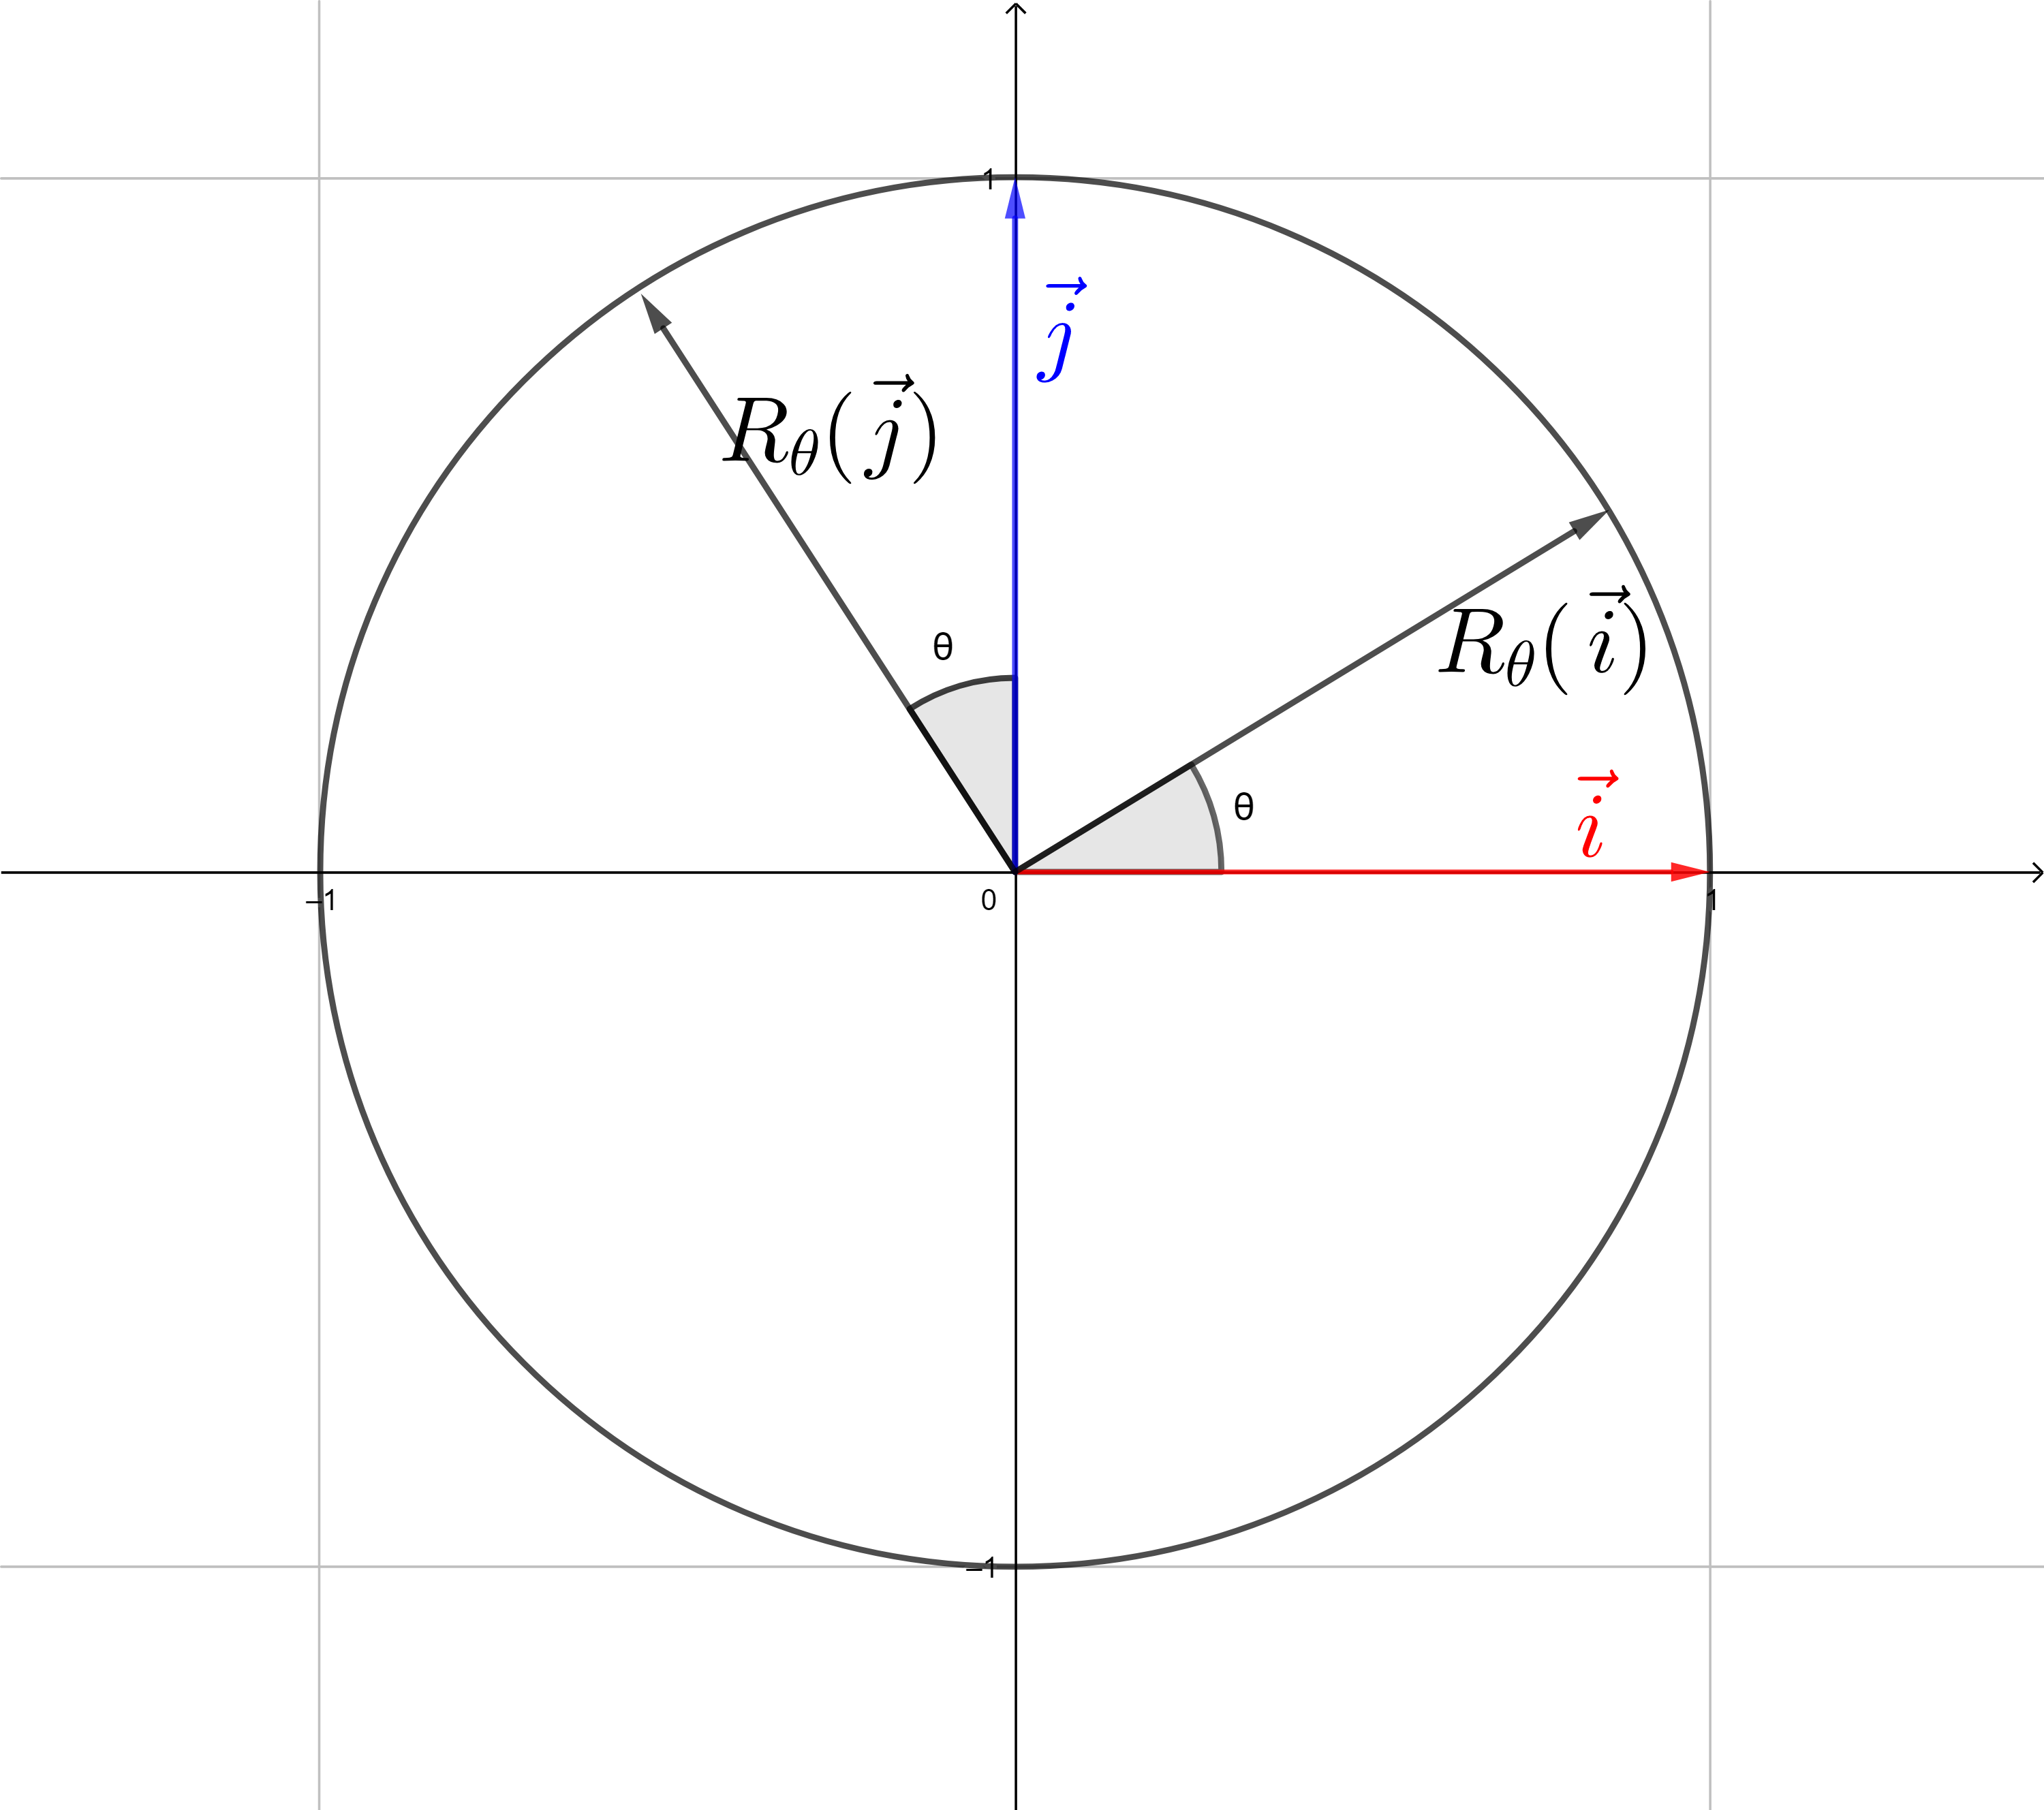
\includegraphics[width=6cm]{rotation.png}
\end{center}
\end{enumerate}
\end{Exemple}
\begin{Proposition}
Si $u$ est une application linéaire alors $u(\vec{0}_E)=\vec{0}_F$.
\end{Proposition}
\begin{Demonstration}
Après simplification de $u(\vec{0}_E)=u(\vec{0}_E+\vec{0}_E)=u(\vec{0}_E)+u(\vec{0}_E)$, on obtient $u(\vec{0}_E)=\vec{0}_F$.
\end{Demonstration}
\begin{Exemple} 
L'application $f(x,y)\mapsto (x+y,1)$ n'est pas linéaire car $f(0,0)=(0,1).$
\end{Exemple}

\begin{Definition}[Endomorphisme]
\begin{itemize}
\item
  Une application linéaire dont l'espace de départ est le même que celui d'arrivée est un \defi{endomorphisme}.
\item
  Un \defi{isomorphisme} est une application linéaire bijective.
\item
  Un \defi{automorphisme} est un endomorphisme bijectif.
\end{itemize}
\end{Definition}
\begin{Exemple}
$\Phi _3$ et $R_\theta$ sont des endomorphismes. Comme $R_\theta$ est bijectif, $R_\theta$ est un automorphisme. 
\end{Exemple}
\begin{DefinitionProposition}[Espace vectoriel des application linéaires et endomorphismes]
Soit $E$ et $F$ deux $\K $-espaces vectoriels.
L'ensemble des applications linéaires de $E$ dans $F$ est noté \defi{$\mathcal{L}(E,F)$} ;
il s'agit d'un sous espace vectoriel de l'espace des fonctions de $E$ dans $F$ muni des lois usuelles.\\
L'espace vectoriel des endomorphismes de $E$ se note \defi{$\LE$}$= \mathcal{L}(E,E)$.
\end{DefinitionProposition}
\begin{Demonstration}
Tous les axiomes se vérifient aisément.  
\end{Demonstration}
\begin{Definition}[composition d'application linéaire]
La \defi{loi de composition interne $\circ$} est définie comme une composition de fonctions, c'est à dire si $u\in\mathcal{L}(E,F)$ et $v\in\mathcal{L}(F,G) $,
 alors  $\forall \vec{x} \in E : (v\circ u)(\vec{x})=v(u(\vec{x}))$.\\
On a $v\circ u\in \mathcal{L}(E,G).$
 \end{Definition}
\begin{Exemple}
L'application $P\mapsto XP'(X^2)$ est un endomorphisme de $\K[X]$. Les applications $P\mapsto P'$, $P\mapsto P(X^2)$ et $P\mapsto XP$ sont linéaire, donc par composition  $P\mapsto XP'(X^2)$ l'est aussi.    
\end{Exemple} 
 \begin{Proposition}[Propriétés]
\begin{itemize}
\item
  \defi{Associativité} : $$(u \circ v) \circ w =u \circ( v \circ w).$$
\item
  \defi{Bilinéarité} : 
  $$ (\lambda u + \mu v) \circ w = \lambda u\circ w + \mu v\circ w\text{ et }u\circ (\lambda v+ \mu w) =\lambda u\circ v + \mu u\circ w.$$
\item
  \defi{Élément neutre} : on appelle \defi{application identité} : $$Id_E:x\mapsto x.$$
 On a $ u\circ Id_E =Id_E\circ u = u.$ 
\end{itemize}
\end{Proposition}
\begin{Demonstration}
La composition des fonctions est associative donc en particulier les fonctions linéaires aussi.\\
Les fonctions sont linéaires à gauche. En revanche, il faut l'hypothèse de linéarité pour la linéarité à droite. En effet, soit $\vec{x}\in E$. On a :
$$u\circ (\lambda v+ \mu w)(\vec{x})=u(\lambda v(\vec{x})+ \mu w(\vec{x}))\overbrace{=}^{\text{linéarité de }u}=\lambda u(v(\vec{x})) + \mu u(w(\vec{x})).$$
\end{Demonstration}

\begin{Remarque} On omet le plus souvent le symbole  $\circ$ : $v\circ u =v u$.
\end{Remarque}
\subsection{Dualité entre le point vue vectoriel et le  point de vue matriciel en dimension finie}
Dans cette sous-section, tous les espaces vectoriels sont de dimension finie.\\
Pour déterminer une application quelconque, on n'a pas d'autre choix que de déterminer les images de chaque point $x\mapsto f(x)$. En revanche,   une application linéaire est complètement déterminer par l'image d'une base. Par exemple, soit $u:(x,y)\mapsto u(x,y)$ une application linéaire avec $u(1,0)=(1,1)$ et $u(0,1)=(1,-1)$. On a 
$$u(x,y)=u(x(1,0)+y(0,1))\overbrace{=}^{\text{linéarité}}x.u(1,0)+ y.u(0,1)=x.(1,1)+ y.u(1,-1)=(x+y,x-y).$$     
\begin{Theoreme}
Pour connaître/définir une application linéaire complètement, il suffit de connaître/définir les  images d'une base de l'espace vectoriel de départ. 
\end{Theoreme}
\begin{Demonstration}[Caractérisation par l'image d'une base]
Soit $\mathcal{B}=(\vec{e_1},\dots,\vec{e_p})$ une base de $E$.\\
Comme $u$ est linéaire, on a :
\begin{align}
u(\vec{x})&=u(\lambda_1.\vec{e_1}+\dots +\lambda_p.\vec{e_p})\\
u(\vec{x})&=\lambda_1.u(\vec{e_1})+\dots +\lambda_p.u(\vec{e_p})
\end{align}
Cela implique que l'application linéaire $u$ est entièrement déterminée par les vecteur $(u(\vec{e_1}),\dots,u(\vec{e_p}))$.
\end{Demonstration}

\begin{Exemple}[Unité pour la proportionnalité]
Il tape au rythme de $42$ mots à la minute. Combien tape-t-il de mot en 10 minutes ?\\
Soit $u$ l'application linéaire représentant le nombre de mot taper en fonction du temps. On a $u(1)=42$. Donc 
$u(10)\overbrace{=}^{\text{linéarité}}10u(1)=420$.
\end{Exemple}

\begin{Definition}[Coordonnées d'un vecteur]
Soit $\mathcal{B} = (\vec{e_1},\dots,\vec{e_p})$ une base de $E$.\\
On sait que tout vecteur $\vec{x}\in  E$ se décompose de façon unique sous la forme
$\vec{x} = x_1 \vec{e_1} + \dots + x_p \vec{e_p}$ où $x_1,\dots, x_p \in   \K$.\\
On appelle coordonnées de $\vec{x}$ dans la base $E$ la matrice colonne
\[ [\vec{x}]_\mathcal{B} = \begin{pmatrix}
x_1\\\vdots\\x_p\\
\end{pmatrix} \]
\end{Definition}
\begin{Remarque}[Identification matrice colonne et $p$-uplets]
On identifiera fréquemment les $p$-uplets avec les matrices colonnes ;
cela est légitime car l'application
\[ \Fonction{\Phi }{\K ^p}{\M{p}{1}{\K}}{(\lambda_1,\dots,\lambda_p)}{\begin{pmatrix}\lambda_1\\\vdots\\\lambda_p\end{pmatrix}} \]
est un isomorphisme.\\
Par exemple, on notera $X=\begin{pmatrix}x_1\\x_2\\\end{pmatrix}\overbrace{=}^{\text{identification}}(x_1,x_2)=\vec{x}.$
\end{Remarque}

\begin{Exemple}[Polynôme] 
Soit $P=1-X^2\in \R_n[X]$. Dans la base canonique $\mathcal{B}=(1,X,X^2,\dots,X^n)$ de $\R_n[X]$, on a $$[P]_\mathcal{B}=\begin{pmatrix}1\\0\\-1\\0\\\vdots \\0\\\end{pmatrix}$$. 
\end{Exemple}
\begin{Definition}[Matrice d'une application linéaire]
Soit $\mathcal{B} = (\vec{e_1},\dots,\vec{e_p})$ une base de $E$ et $\mathcal{B}' = (\vec{f_1},\dots,\vec{f_n})$ une base de $F$.
Pour tout $j\in  \{1,\dots,p\}$, le vecteur $u(\vec{e_j})$ se décompose dans la base $\mathcal{B}'$:
\[u(\vec{e_j})=a_{1j}.\vec{f_1}+\dots +a_{nj}.\vec{f_n}. \]
On appelle \defi{matrice de l'application linéaire $u$} la matrice, $[u]_\mathcal{B}^{\mathcal{B}'}$,  définie par :
\begin{center}
  \begin{tikzpicture}[
      every left delimiter/.style={xshift=0.75em},
      every right delimiter/.style={xshift=-0.75em},
      dots/.style={
        line width=1pt,
        line cap=round,
        dash pattern=on 0pt off 5pt,
        shorten >=.1cm,
    shorten <=.1cm}]
    \matrix (M) [
      matrix of nodes,
      left delimiter=(,
      right delimiter=),
    ]{
      \node (A) {$a_{11}$}; &[1.1cm] \node (B) {$a_{1p}$}; \\[1.1cm]
      \node (C) {$a_{n1}$}; &        \node (D) {$a_{np}$}; \\
    };

    \draw (M.west) node[left] {$[u]_\mathcal{B}^{\mathcal{B}'}=$};
    \draw [dots] (A.east)  -- (B.west);
    \draw [dots] (C.east)  -- (D.west);
    \draw [dots] (A.south) -- (C.north);
    \draw [dots] (B.south) -- (D.north);
    \draw (A) [yshift=0.7cm] node (E) {$u(\vec{e_1})$};
    \draw (B) [yshift=0.7cm] node (F) {$u(\vec{e_p})$};
    \draw (B) [xshift=1cm]   node (G) {$\vec{f_1}$};
    \draw (D) [xshift=1cm]   node (H) {$\vec{f_n}$};
    \draw [dots] (E.east)  -- (F.west);
    \draw [dots] (G.south) -- (H.north);
  \end{tikzpicture}
\end{center}
Les autres notations sont $ [u]_\mathcal{B}^{\mathcal{B}'}= \mat(u,\mathcal{B} \to \mathcal{B}') = \mat_{\mathcal{B}\to\mathcal{B}'}(u).$\\
Dans le cas d'un endomorphisme, $E=F$  et $\mathcal{B}=\mathcal{B}'$, on la note $[u]_\mathcal{B}$ ou $\mat(u,\mathcal{B})$ ou $\mat_\mathcal{B}(u)$.
\end{Definition}
\begin{Exemple}[Dérivée polynomial] La matrice de $\Fonction{\Phi _3}{\mathbb {R}_n[X] }{\mathbb {R}_n[X]}{P}{P'}$ dans la base canonique $\mathcal{B}=(1,X,X^2,\dots,X^n)$ est :
 $$[\Phi _3]_{\mathcal{B}}= \begin{pmatrix} 0 &1&0&\ldots &0 \\
 0& 0&2&\ddots \\
 \vdots &  &\ddots & \ddots \\
  \vdots &  & & \ddots& n\\
 0 &  & \dots& & 0
\end{pmatrix}   $$
car $\Phi _3(X^i)=i X^{i-1}$.
\end{Exemple}
\begin{Theoreme}[Dualité]
Soit $\mathcal{B}$ une base de $E$ et $\mathcal{B}'$ une base de $F$.\\
L'application
\[ \Fonction{\Phi}{\mathcal{L}(E,F)}{\M{n}{q}{\K} }{u}{[u]_\mathcal{B}^{\mathcal{B}'}} \]
est linéaire et bijective, autrement dit un isomorphisme.
\end{Theoreme}
\begin{Demonstration}
On ajoute une seconde partie à la démonstration sur la caractérisation d'une application linéaire par l'image d'une base.\\
Soit $\mathcal{B}'=(\vect{f_1},\dots,\vect{f_n})$ une base de $F$.\\
Il existe une famille $(a_{ij})_{\substack{1\leq i\leq n\\1\leq j\leq p}}$ d'éléments de $\K$ tel que :
$$\forall j\in \Intf{1}{p}: u(\vect{e_j})=a_{1j}\vect{f_1}+\dots+a_{nj}\vect{f_n}.$$ 
Ainsi, les coefficient $(a_{ij})_{\substack{1\leq i\leq n\\1\leq j\leq p}}$ de la matrice $[u]_\mathcal{B}^{\mathcal{B}'}$   caractérise entièrement l'application linéaire $u$ d'où l'isomorphisme. 
\end{Demonstration}

\begin{Corollaire}[Dimension de $\mathcal{L}(E,F)$]
$$\dim \mathcal{L}(E,F) = \dim(E) \times\dim(F).$$
\end{Corollaire}
\begin{Demonstration}
Comme l'application $\Phi$ est bijective, la dimension de l'espace vectoriel de départ est égale à celle d'arrivé (voir la section image et noyau). Donc on a $$\dim \mathcal{L}(E,F)=\dim \M{n}{q}{\K}= n q= \dim (F)\dim (E).$$ 
\end{Demonstration}

\begin{DefinitionProposition}[Application linéaire d'une matrice]
Inversement, si l'on se donne une matrice $M \in   \M{n}{q}{\K} $,
on peut définir une application linéaire, dite \defi{canoniquement associée à $M$}, par
\[ \Fonction{u_M}{\M{p}{1}{\K}}{\M{n}{1}{\K}}{X}{M\times X}.\]
Si l'on note $\mathcal{B}$ la base canonique de $\M{p}{1}{\K}$ et $\mathcal{B}'$ la base canonique de $\M{n}{1}{\K}$,
on vérifie  que
\[ [u_M]_{\mathcal{B}}^{\mathcal{B}'} = M. \]
\end{DefinitionProposition}
\begin{Demonstration}
$u_M$ est  une application linéaire car $$u_M(X+Y)= M\times(X+Y)=M\times X + M\times Y=u_M(X)+u_M(Y)$$ et $$u_M(\lambda X)=M\times(\lambda X)=\lambda M\times X=\lambda u_M( X).$$ 
\end{Demonstration}
\begin{Exemple}[Matrice de rotation]
La matrice de rotation $\begin{pmatrix}\cos \theta & -\sin \theta\\ \sin \theta & \cos \theta\end{pmatrix}$ est canoniquement associée à l'application linéaire rotation $\Fonction{R_\theta}{\mathbb {R}^2 }{\mathbb {R}^2}{(x,y)}{ (x\cos \theta - y \sin \theta,x\sin \theta + y \cos \theta)}$ en ayant effectuée l'identification de $\R^2$ avec $\M{2}{1}{\K}$. 
\end{Exemple}


\begin{Theoreme}[Image d'une application linéaire et image d'une matrice]
Soit $\mathcal{B}$ une base de $E$ et $\mathcal{B}'$ une base de $F$.\\
Soit $u:E\to F$ une application linéaire et $\vec{x}$ un vecteur de $E$.\\
Alors \[ [u(\vec{x})]_{\mathcal{B}'} = [u]_\mathcal{B}^{\mathcal{B}'} × [\vec{x}]_\mathcal{B}. \]
ou si on pose $Y=[u(\vec{x})]_{\mathcal{B}'},\quad A =[u]_\mathcal{B}^{\mathcal{B}'}$ et  $[\vec{x}]_\mathcal{B}$, on a :
$$Y=AX.$$
\end{Theoreme}
\begin{Demonstration}
Soit $\mathcal{B}=(\vect{e_1},\dots,\vect{e_p})$ une base de $E$.\\
Soit $\mathcal{B}'=(\vect{f_1},\dots,\vect{f_n})$ une base de $F$.\\
Soit $(a_{ij})_{\substack{1\leq i\leq n\\1\leq j\leq p}}$ les coefficients de la matrice $[u]_\mathcal{B}^{\mathcal{B}'}$.\\
Soit $\vec{x}=x_1\vect{e_1}+\dots+x_p\vect{e_p}\in E$.\\
On a :
$$u(\vec{x})\overbrace{=}^{\text{linéarité}} =\sum_{j=1}^p x_j\vect{e_j}=\sum_{j=1}^p x_j\sum_{i=1}^n a_{ij} \vect{f_i}=\sum_{i=1}^n \left(\sum_{j=1}^p x_j a_{ij}\right) \vect{f_i}, $$
d'où $ [u(\vec{x})]_{\mathcal{B}'}=\begin{pmatrix}\sum_{j=1}^p x_j a_{1j} \\\vdots\\\sum_{j=1}^p x_j a_{nj} \end{pmatrix}$.\\
Aussi on a :

$$\begin{aligned}\\
 &\begin{pmatrix}x_1\\\vdots\\x_p\end{pmatrix} \\
\left[u\right]_{\mathcal{B}}^{\mathcal{B}'} \times \left[\vec{x}\right]_{\mathcal{B}}=\begin{pmatrix}
    a_{11} &  \dots & a_{1p}  \\
    \vdots &   &  \vdots  \\
    a_{n1} &  \dots & a_{np}
  \end{pmatrix}& \\
\left[u\right]_{\mathcal{B}}^{\mathcal{B}'} \times \left[\vec{x}\right]_{\mathcal{B}}=\begin{pmatrix}\sum_{j=1}^p x_j a_{1j} \\\vdots\\\sum_{j=1}^p x_j a_{nj} \end{pmatrix}&.
\end{aligned}$$
Finalement on obtient bien $ [u(\vec{x})]_{\mathcal{B}'} = [u]_\mathcal{B}^{\mathcal{B}'} × [\vec{x}]_\mathcal{B}. $
\end{Demonstration}

\begin{Exemple}[Dérivée polynomial] 
Soit $P=1-X^2$. On a $[P]_\mathcal{B}=\begin{pmatrix}1\\0\\-1\\0\\\vdots \end{pmatrix}$. D'où 
$$[\Phi_3(P)]_\mathcal{B}=  [\Phi _3]_{\mathcal{B}} [P]_\mathcal{B} =\begin{pmatrix} 0 &1&0&\ldots &0 \\
 0& 0&2&\ddots \\
 \vdots &  &\ddots & \ddots \\
  \vdots &  & & \ddots& n\\
 0 &  & \dots& & 0
\end{pmatrix}  \begin{pmatrix}1\\0\\-1\\0\\\vdots \end{pmatrix} = \begin{pmatrix}0\\-2\\0\\0\\\vdots \end{pmatrix}    $$
D'où le résultat escompté $\Phi_3(P)=-2X$.
\end{Exemple}

\begin{Theoreme}[Produit matriciel et composition d'applications linéaires]
Soit $E$, $F$, $G$ trois espaces vectoriels de dimension finie munis des bases respectives $\mathcal{B}$, $\mathcal{B}'$ et $\mathcal{B}''$.\\
Soit $u:E\to F$ et $v:F\to G$ deux applications linéaires.\\
Alors
\[  [v\circ u]_{\mathcal{B}}^{\mathcal{B}''} = [v]_{\mathcal{B}'}^{\mathcal{B}''} ×[u]_{\mathcal{B}}^{\mathcal{B}'}. \]
\end{Theoreme}
En résumé, si l'espace vectoriel de départ est le même que celui d'arrivée, avec $\mathcal{B}=(\vec{e}_1, \dots  ,\vec{e}_n)$ base de $E$, nous avons :\\
\begin{center}
\begin{tabular}{c|c|c}
Vectoriel &  &Matriciel \\
\hline\hline
$\vec{x}=x_1.\vec{e}_1+ \dots  +x_n.\vec{e}_n \in E$& $\longrightarrow$ & $X=[\vec{x}]_{\mathcal{B}}=\begin{pmatrix}x_1\\ \vdots\\x_n\end{pmatrix}\in\M{n}{1}{\K} $ \\\hline
$u\in\mathcal{L}(E)$ &$\longrightarrow$    & \begin{tikzpicture}[
      every left delimiter/.style={xshift=0.75em},
      every right delimiter/.style={xshift=-0.75em},
      dots/.style={
        line width=1pt,
        line cap=round,
        dash pattern=on 0pt off 5pt,
        shorten >=.1cm,
    shorten <=.1cm}]
    \matrix (M) [
      matrix of nodes,
      left delimiter=(,
      right delimiter=),
    ]{
      \node (A) {$a_{11}$}; &[1.1cm] \node (B) {$a_{1n}$}; \\[1.1cm]
      \node (C) {$a_{n1}$}; &        \node (D) {$a_{nn}$}; \\
    };

    \draw (M.west) node[left] {$A=[u]_\mathcal{B}=$};
    \draw [dots] (A.east)  -- (B.west);
    \draw [dots] (C.east)  -- (D.west);
    \draw [dots] (A.south) -- (C.north);
    \draw [dots] (B.south) -- (D.north);
    \draw (A) [yshift=0.7cm] node (E) {$u(\vec{e_1})$};
    \draw (B) [yshift=0.7cm] node (F) {$u(\vec{e_n})$};
    \draw (B) [xshift=1cm]   node (G) {$\vec{e_1}$};
    \draw (D) [xshift=1cm]   node (H) {$\vec{e_n}$};
    \draw [dots] (E.east)  -- (F.west);
    \draw [dots] (G.south) -- (H.north);
  \end{tikzpicture}\\\hline
$\vec{y}=y_1.\vec{e}_1+ \dots  +y_n.\vec{e}_n=u(\vec{x})$&$\longrightarrow$ & $Y=[\vec{y}]_{\mathcal{B}}=\begin{pmatrix}y_1\\ \vdots\\y_n\end{pmatrix}=A\times X $ \\\hline
 $u\circ v $ avec $u,v \in\mathcal{L}(E)$ &$\longrightarrow$ &  $[u\circ v]_{\mathcal{B}} =A\times B$ avec $A=[u]_\mathcal{B}$ et $B=[v]_\mathcal{B}$\\
%$\ker u = \{\vec{x}\in E:u(\vec{x}) = \vec{0}\} $      &$\longrightarrow$ &$\ker [u]_\mathcal{B}= \{X:[u]_\mathcal{B} X = 0\}$ \\\hline
%$\im u = \{u(\vec{x}):\vec{x}\in E\} $      & $\longrightarrow$&$\im [u]_\mathcal{B}= \{[u]_\mathcal{B} X:X\in \M{M}{n,1}{\K}\}$\\\hline
\hline

$\Fonction{u_M}{ \M{n}{1}{\K}}{ \M{n}{1}{\K}}{X}{M\times X}\in\mathcal{L}(\M{n}{1}{\K})   $ &$\longleftarrow $ & $M\in \M{n}{n}{\K}$
 
\end{tabular}
 \end{center}
L'annexe~\ref{subsec:dualite} présente le lien entre le point de vue vectoriel $\vec{y}=u(\vec{x})$) et  le point de vue matricielle.

\subsection{Endomorphisme/Matrice carré}

\begin{Definition}[Structure d'algèbre des endomorphismes]
L'\defi{élément neutre} de la composition dans $\LE$ est l'application identité, $\mathrm {Id}_{E}:x\mapsto x$. L'endomorphisme $u^{-1}$ est appelé l' \defi{endomorphisme inverse} de $u$ si $ u^{-1}×u=u×u^{-1}=\mathrm {Id}_{E}$. Dans ce cas, l'endomorphisme $u$ est dite \defi{inversible}.  $\LE$ possède une structure d'algèbre non commutative. L'espace vectoriel des automorphismes de $E$ se note $ \GLE$.   $(\GLE,\circ)$ est un groupe, appelé \defi{groupe linéaire}.
\end{Definition}
\begin{Definition}[Structure d'algèbre des matrices carrés]
L'\defi{élément neutre} de la multiplication dans l'ensemble des matrices carrés $\MnK$ est la matrice identité, $\mathrm {I} _{n}$, avec des 1 sur la diagonale et des 0 partout ailleurs.  
$$ \mathrm {I} _{n}=\begin{pmatrix}1&0&\cdots &0\\0&\ddots &\ddots &\vdots \\\vdots &\ddots &\ddots &0\\0&\cdots &0&1\end{pmatrix}.$$Soit $A\in\MnK$. La matrice $A^{-1}$ est appelé la \defi{matrice inverse} de $A$ si $ A^{-1}×A=A×A^{-1}= \mathrm {I} _{n}$. Dans ce cas, la matrice $A$ est dite \defi{inversible}.  $\MnK$ possède une structure d'algèbre non commutative. L'espace vectoriel des matrice inversibles de taille $n$ se note $\GLnK$.   $(\GLnK,\times)$ est un groupe, appelé \defi{groupe linéaire}.  
\end{Definition}
\begin{Proposition}[Dualité]
Soit $E$ un espace vectoriel de dimension $n$. Soit $\mathcal{B}$ une base de $E$.\\
$$u\in\GLE\Leftrightarrow [u]_\mathcal{B}\in \GLnK.$$
Aussi, soit $M$ une matrice carré.
$$M \in \GLnK \Leftrightarrow u_M\in \GLE[\K^n] .$$
\end{Proposition}
%TODO mettre un exemple
\section{Image et noyau}
\subsection{Généralités}
Soit $u:E\to F$ une application linéaire.\\
Soit $M\in\M{p}{n}{K}$.
\begin{Definition}[Image directe et image réciproque]
Soit $f:A\to B$. Soit $A'$ une partie de $A$ et $B'$ une partie de $B$.\\
L'ensemble $\{f(x): x  \in  A'\}$ est appelé \defi{image directe} de $A'$ par $f$ et noté $f(A')$.\\
L'ensemble $\{x\in A : f(x)  \in  B'\}$ est appelé \defi{image réciproque} de $B'$ par $f$ et noté $f^{-1}(B')$.\\
\end{Definition}
\begin{Exemple}[Carré]
Soit $f:x\mapsto x^2$.\\
On a $f([-1,1])=[0,1]$ et $f^{-1}(\{2\})=\{-\sqrt{2},\sqrt{2}\}$.
\end{Exemple}
\begin{Proposition}[Morphisme d'espace vectoriel]
Soit $E',F'$ deux sous-espace vectoriel de de $E$ et $F$ respectivement.\\
\begin{itemize}
\item $u(E')$ est un sous espace vectoriel de $F$,
\item $u^{-1}(F')$ est un sous espace vectoriel de $E$.
\end{itemize}
\end{Proposition}
\begin{Remarque}
En particulier pour l'application linéaire associée à $M$,  $u_M(E')$ est un sous espace vectoriel de $\M{n}{1}{\K}$ et $u_M^{-1}(F')$ est un sous espace vectoriel de $\M{p}{1}{\K}$.
\end{Remarque}
\begin{Proposition}
Soit $(\vec{x_i})_{i\in I}$ une famille de $E$ .\\
Alors $$ u(\text{Vect}((\vec{x_i})_{i\in I}))=\text{Vect}( \left(u(\vec{x_i})\right)_{i\in I})).$$
\end{Proposition}
\begin{Exemple}
L'image de la droite vectoriel $\R (1,1)$ par $R_\theta$ est la droite vectoriel $\R R_\theta(1,1)$.
\end{Exemple}
\begin{Definition}[Noyau et image]
\begin{itemize}
\item
  L'\defi{image} de $u$ est le sous espace vectoriel $u(E) = \{u(\vec{x}):\vec{x}\in  E\}$;
  on le note $\im u$.
\item
  Le \defi{noyau} de $u$ est le le sous espace vectoriel $u^{-1}\{ \{\vec{0_F}\}\} = \{x\in  E:u(\vec{x}=\vec{0_F}\}$;
  on le note $\Ker u$.
\end{itemize}
\end{Definition}
\begin{Proposition}[Image d'une base]
Soit $(\vec{e_i})_{i\in I}$ une base de $E$ .\\
Alors $$ \Ima u =\text{Vect}( \left(u(\vec{x_i})\right)_{i\in I})).$$
\end{Proposition}

\begin{Exemple}\label{ex:noyau}
Soit $\Fonction{u}{\R^3}{\R^2}{(x,y,z)}{(x+y+z,x-y)}$.\\
On a $u(x,y,z)=x(1,1)+y(1,-1)+z(0,1)$.
Donc $\Ima u$ est l'espace vectoriel engendré par la famille $((1,1),(1,-1),(0,1))$ d'où $\Ima u=\R^2$.
$$(x,y,z)\in \Ker u \Leftrightarrow u(x,y,z)=(0,0)  \Leftrightarrow \begin{cases}x+y+z=&0\\x-y=&0\end{cases}\overbrace{\Leftrightarrow}^{x=t} \exists t \in \R: (x,y,z)=t(1,1,-2).$$
Donc $\Ker u =\R (1,1,2).$
\end{Exemple}
\begin{Exemple}[Dérivée polynomiale]
Soit $P=a_0+a_1 X+\dots + a_n X^n \in \R_n[X].$
On a $\Phi_3(P)=P'=a_1+a_2 .2X+\dots  + a_n.nX^{n-1}$.
Donc $\Ima \Phi_3$ est l'espace vectoriel engendré par la famille $(1,X,2X,\dots,nX^{n-1})$, soit $\Ima \Phi_3=\R_{n-1}[X].$
 $$P\in \Ker \Phi_3  \Leftrightarrow \Phi_3(P)=0  \Leftrightarrow P'=0\Leftrightarrow \exists a\in \R : P=a.$$
Donc $\Ker \Phi_3 =\R_{0}[X].$
\end{Exemple}
\begin{Definition}[Noyau et image]
\begin{itemize}
\item
  L'\defi{image} de $M$ est le sous espace vectoriel $u_M(\M{n}{1}{\K}) = \{MX:X\in \M{n}{1}{\K}\}$;
  on le note $\im M$.
\item
  Le \defi{noyau} de $M$ est le le sous espace vectoriel $u_M^{-1}\{ \{0 \}\} = \{X\in  \M{n}{1}{\K}:MX=0\}$;
  on le note $\Ker M$.
\end{itemize}
\end{Definition}

\begin{Exemple}
Soit $M=\begin{pmatrix}
1&1&1\\
1&-1&0\\
\end{pmatrix}$
On a $M\begin{pmatrix}x \\y \\z\\\end{pmatrix}=x\begin{pmatrix}1\\1\\ \end{pmatrix}+y\begin{pmatrix}1\\-1\\ \end{pmatrix}+z\begin{pmatrix}0\\1\\ \end{pmatrix}$.
Donc $\Ima M$ est l'espace vectoriel engendré par la famille $(\begin{pmatrix}1\\1\\ \end{pmatrix},\begin{pmatrix}1\\-1\\ \end{pmatrix},\begin{pmatrix}0\\1\\ \end{pmatrix})$ d'où $\Ima M=\M{2}{1}{\K}$.
$$\begin{pmatrix}x \\y \\z\\\end{pmatrix} \in \Ker M \Leftrightarrow M\begin{pmatrix}x \\y \\z\\\end{pmatrix}=\begin{pmatrix}0 \\0 \\0\\\end{pmatrix} \Leftrightarrow \begin{cases}x+y+z=&0\\x-y=&0\end{cases}\overbrace{\Leftrightarrow}^{x=t} \exists t \in \R: \begin{pmatrix}x \\y \\z\\\end{pmatrix}=t\begin{pmatrix}1 \\1 \\-2\\\end{pmatrix} .$$
Donc $\Ker M =\R \begin{pmatrix}1 \\1 \\-2\\\end{pmatrix}.$\\
Comme $M$ est la matrice associée à l'application linéaire de l'exemple~\ref{ex:noyau}, on retrouve les mêmes résultats en identifiant les n-uplets aux matrices colonnes. 
\end{Exemple}
\begin{Proposition}[Image d'une base]
L'image d'une matrice est l'espace vectoriel engendré par ses colonnes.
\end{Proposition}
\begin{Definition}[Rang] Le \defi{rang} d'une  application linéaire $u$ est  la dimension de l'espace vectoriel $\Ima u$.\\
Le \defi{rang} d'une matrice est le rang de l'application linéaire canoniquement associée.
\end{Definition}
\begin{Proposition} Le \defi{rang} d'une matrice est le rang de la famille de ses vecteurs colonnes. 
\end{Proposition}
\begin{Proposition}[injective et surjective caractérisations]  
\begin{itemize}
\item
  $u$ est injective si et seulement si $\Ker u = \{\vec{0_E}\}$,
\item
  $u$ est surjective si et seulement si $\Ima u = F$.
\end{itemize}
\end{Proposition}
\begin{Proposition}
Si $u$ est bijective, alors $u^{-1}$ est également linéaire.
\end{Proposition}
\begin{Proposition}[Dualité]
Soit $E$ un espace vectoriel de dimension n. Soit $\mathcal{B}$ une base de $E$. 
\begin{center}
$u$ est injective si et seulement si $\Ker [u]_\mathcal{B}= \{0\}$.
\end{center}   
\end{Proposition}
\subsection{Effet d'une applications linéaire sur la dimension}
Une application linéaire, $u:E\to F$ ne peut que réduire la dimension de son ensemble de définition. 
\begin{center}
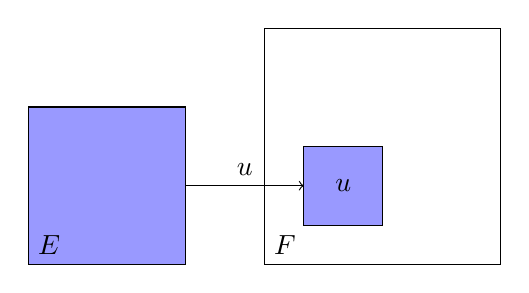
\begin{tikzpicture}
\fill[blue!40!white, draw=black] (0,0) rectangle (2,2);
\draw  (0,0) node[above right]{$E$};
\fill[white, draw=black] (3,0) rectangle (6,3);
\draw  (3,0) node[above right]{$F$};
\fill[blue!40!white, draw=black] (3.5,0.5) rectangle (4.5,1.5);
\draw  (4,1) node{$\im u$};
\draw[->]  (2,1) --node[above]{$u$} (3.5,1) ;
\end{tikzpicture}
\end{center}
L'application est injective si et seulement si: $\rg u =\dim E$.
\begin{center}
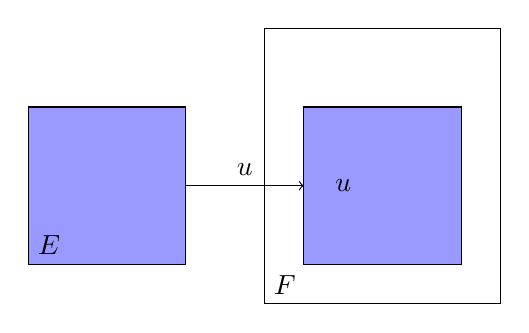
\begin{tikzpicture}
\fill[blue!40!white, draw=black] (0,0) rectangle (2,2);
\draw  (0,0) node[above right]{$E$};
\fill[white, draw=black] (3,-0.5) rectangle (6,3);
\draw  (3,-0.5) node[above right]{$F$};
\fill[blue!40!white, draw=black] (3.5,0) rectangle (5.5,2);
\draw  (4,1) node{$\im u$};
\draw[->]  (2,1) --node[above]{$u$} (3.5,1) ;
\end{tikzpicture}
\end{center}
L'application est surjective si et seulement si: $\rg u =\dim F$.
\begin{center}
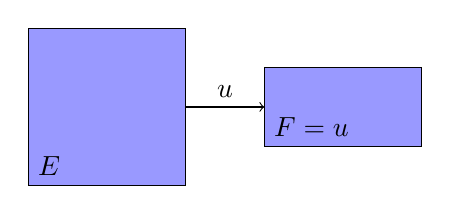
\begin{tikzpicture}
\fill[blue!40!white, draw=black] (0,0) rectangle (2,2);
\draw  (0,0) node[above right]{$E$};
\fill[blue!40!white, draw=black] (3,0.5) rectangle (5,1.5);
\draw  (3,0.5) node[above right]{$F=\im u$};
\draw[->]  (2,1) --node[above]{$u$} (3,1) ;
\end{tikzpicture}
\end{center}
L'application est bijective si et seulement si: $\rg u =\dim F=\dim E$.
\begin{center}
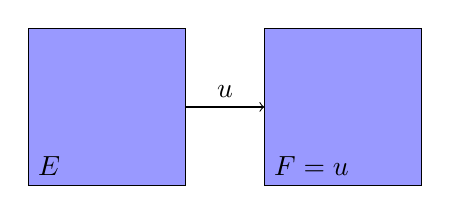
\begin{tikzpicture}
\fill[blue!40!white, draw=black] (0,0) rectangle (2,2);
\draw  (0,0) node[above right]{$E$};
\fill[blue!40!white, draw=black] (3,0) rectangle (5,2);
\draw  (3,0) node[above right]{$F=\im u$};
\draw[->]  (2,1) --node[above]{$u$} (3,1) ;
\end{tikzpicture}
\end{center}
\begin{Proposition}[Inégalité et égalité sur le rang]
Soit $u:E\to F$ une application linéaire.
\begin{enumerate}
\item Si $F$ est de dimension finie, $\rg u \leq \dim F$, avec égalité si et seulement si $u$ est surjective.
\item  Si $E$ est de dimension finie, $\rg u \leq \dim E$, avec égalité si et seulement si $u$ est injective.
\end{enumerate}
\end{Proposition}
\begin{Proposition}[Cas $\dim E = \dim F$]
Soit $u:E\to F$ une application linéaire tel que $\dim E = \dim F$.
\begin{center}
$u$ est bijective $\Leftrightarrow$ $u$ est injective $\Leftrightarrow$ $u$ est surjective.
\end{center}
Soit $u:E\to E$ une application linéaire tel que $\dim E$ est finie.
\begin{center}
\begin{tabular}{ccccc}
$u$ est bijective& $\Leftrightarrow$& $u$ est injective &$\Leftrightarrow$ &$u$ est surjective \\
$u\in \mathcal{GL}(E)$ &$\Leftrightarrow$ &  $u$ est inversible à gauche &$\Leftrightarrow$ &  $u$ est inversible à droite \\
$\exists v\in \mathcal{L}(E): u\circ v =v \circ u = \mathrm{Id}_E$ &$\Leftrightarrow$ &  $\exists v\in \mathcal{L}(E): v\circ u= \mathrm{Id}_E$  &$\Leftrightarrow$ &  $\exists v\in \mathcal{L}(E): u\circ v= \mathrm{Id}_E$
\end{tabular}
\end{center}
\end{Proposition}
\begin{Exemple}
Démontrons que l'application linéaire $u:(x,y)\to (x+y,x-y)$ est bijective.\\
Comme $u$ est un endomorphisme, il suffit de démontrer qu'elle est injective.\\
$$(x,y)\in \Ker u \Leftrightarrow \begin{cases}x+y=0\\x-y=0\end{cases}  \Leftrightarrow  \begin{cases}x=0\\y=0\end{cases} $$ 
Donc $\Ker u =\{(0,0)\}.$
\end{Exemple}
\begin{Exemple}
Démontrons que l'application linéaire $u:P\to P-P'$ est bijective sur $\R_n[X]$.\\
Comme $u$ est un endomorphisme, il suffit de montrer qu'elle est injective.\\
$$P\in \Ker u \Leftrightarrow P-P'=0  \Leftrightarrow  P=P'$$ 
Donc $\Ker u =\{0\}$ car $\deg(P)=\deg(P')$ si et seulement $P=0$.
\end{Exemple}
\begin{Proposition}[Inversibilité à gauche et à droite d'une matrice carré]
Soit $A,B\in \MnK$.
Si $AB=I_n$ alors $A$ et $B$ sont toutes deux inversibles et inverses l'une de l'autre.
\end{Proposition}
\subsection{Théorème du rang : $\dim E = \Rang u + \dim \Ker u$}
Les dimensions du noyau et l'image d'une application linéaire sont liées.\\
Soit $A=\begin{pmatrix} 1 &  0 &1\\ 0 &1 &1\\ 0 &1&1\end{pmatrix}$. On a $C_3=C_1+C2$.\\
\textit{Image}  : $\im(A)=\mathrm{Vect}(C_1,C_2,C_3)\overbrace{=}^{C_3=C_1+C2}\mathrm{Vect}(C_1,C_2).$ Comme les vecteur $C_1$ et $C_2$ sont linéairement indépendants, $\dim (\im(A))=2$.\\
\textit{Noyau}  : $\begin{pmatrix}x\\y\\z \end{pmatrix}\in \Ker(A)\Leftrightarrow xC_1 + yC_2 + zC_3= 0\overbrace{\Leftrightarrow}^{C_3=C_1+C2} (x+z)C_1 + (y+z)C_2 = 0$ \\$ \overbrace{\Leftrightarrow}^{C_1,C_2\text{linéairement indépendants} }\begin{cases}x=-z\\y=-z\end{cases} \Leftrightarrow \Ker(A)= \mathrm{Vect} \begin{pmatrix}1\\1\\-1 \end{pmatrix}$. Donc $\dim (\Ker(A))=1$.\\
On observe que $\dim \Ker A +\dim \im A =$taille de la matrice. 


\begin{Proposition}[Factorisation]
Soit $E$ et $F$ deux $\K $-espaces vectoriels  et $u:E\to F$ une application linéaire.
Si $S$ est un supplémentaire de $\Ker u$, alors $u$ induit un isomorphisme de $S$ sur $\Ima u$,
c'est à dire que l'application linéaire
\[ \Fonction{v}{S}{\Ima u}{\vec{x}}{u(\vec{x})} \]
est bijective.
\end{Proposition}
\begin{Theoreme}[Théorème du rang]

Soit $E$ et $F$ deux $\K $-espaces vectoriels  et $u:E\to F$ une application linéaire.
On suppose que $E$ est de dimension finie.
Alors $\Ima u$ est de dimension finie et
\[ \dim E = \Rang u + \dim \Ker u. \]
\end{Theoreme}
\begin{Theoreme}[Théorème du rang version matricielle]

Soit $M \in   \M{n}{q}{\K} $.

Alors 
\[ p = \Rang M + \dim \Ker M. \]
\end{Theoreme}
%% ---------------------------------------------------------------------------
\section{Changement de base}
Il faut bien garder à l'esprit que la matrice d'une application linéaire est une "représentation"
de celle-ci qui dépend du choix des bases au départ et à l'arrivée. Il est utile de savoir passer
d'une représentation à une autre. Connaissant la matrice d'une application linéaire dans deux
bases, il faut savoir la déterminer dans deux autres bases.
\subsection{D'une représentation à l'autre}
\begin{Definition}[Matrice de passage]
Soit $E$ un espace vectoriel de dimension finie et  $\mathcal{B}$ et $\mathcal{B}'$ deux bases de $E$.
On appelle \defi{matrice de passage} de $\mathcal{B}$ à $\mathcal{B}'$ la matrice
\[ P_{\mathcal{B}\to\mathcal{B}'} = [\mathrm{Id}_E]_{\mathcal{B}'}^{\mathcal{B}}. \]

De façon plus explicite, notons $\mathcal{B} = \{\vec{e_1},\dots,\vec{e_n}\}$,
$\mathcal{B}' = \{\vec{f_1},\dots,\vec{f_n}\}$ et $P_{\mathcal{B}\to\mathcal{B}'} = ( a_{ij} )_{1\leq i \leq n,1\leq j \leq n}$.
Dans ce cas, on a
\[ \forall   j \in   \{1,\dots,n\}:\quad \vec{f_j} = \sum  _{i=1}^n a_{ij} \vec{e_i}. \]
Ainsi,
\begin{center}
  \begin{tikzpicture}[
      every left delimiter/.style={xshift=0.75em},
      every right delimiter/.style={xshift=-0.75em},
      dots/.style={
        line width=1pt,
        line cap=round,
        dash pattern=on 0pt off 5pt,
        shorten >=.1cm,
    shorten <=.1cm}]
    \matrix (M) [
      matrix of nodes,
      left delimiter=(,
      right delimiter=),
    ]{
      \node (A) {$a_{11}$}; &[1.1cm] \node (B) {$a_{1n}$}; \\[1.1cm]
      \node (C) {$a_{n1}$}; &        \node (D) {$a_{nn}$}; \\
    };

    \draw (M.west) node[left] {$P_{\mathcal{B}\to\mathcal{B}'}=$};
    \draw [dots] (A.east)  -- (B.west);
    \draw [dots] (C.east)  -- (D.west);
    \draw [dots] (A.south) -- (C.north);
    \draw [dots] (B.south) -- (D.north);
    \draw (A) [yshift=0.7cm] node (E) {$\vec{f_1}$};
    \draw (B) [yshift=0.7cm] node (F) {$\vec{f_n}$};
    \draw (B) [xshift=1cm]   node (G) {$\vec{e_1}$};
    \draw (D) [xshift=1cm]   node (H) {$\vec{e_n}$};
    \draw [dots] (E.east)  -- (F.west);
    \draw [dots] (G.south) -- (H.north);
  \end{tikzpicture}
\end{center}
\end{Definition}
\begin{Proposition}[Inversible]
Si $P$ est une matrice de passage alors $P$ est inversible.\\
Si  $P$ est inversible alors $P$ est la matrice de passage de la base canonique à la base de ses colonnes $(C_1,\dots, C_n)$.
\end{Proposition}


 \begin{Exemple}
Dans $\R ^2$, si $\mathcal{B}$ est la base canonique et si $\mathcal{B}' = \left( \begin{pmatrix}
1\\2
\end{pmatrix},\begin{pmatrix}
-1\\3
\end{pmatrix}\right) $, alors :\\
$P_{\mathcal{B}\to\mathcal{B}'}=\begin{pmatrix}
1&-1\\2&3
\end{pmatrix}$et $P_{\mathcal{B}'\to\mathcal{B}}=\begin{pmatrix}
\frac 35&\frac 15\\-\frac 25&\frac 15
\end{pmatrix}$
La première matrice de passage ne nécessite aucun calcul, la seconde résulte de la méthode du Pivot de Gauss:
$$\begin{array}{rl}
&\left({\begin{array}{rr|rr}1 &-1& 1 & 0\\ 2 & 3 &0&1 \end{array}}\right)\\
\begin{small}\begin{array}{r} \\(L2)\leftarrow (L2)-2(L1) \end{array}\end{small}&\left({\begin{array}{rr|rr}1 &-1& 1 & 0\\ 0 & 5 &-2&1 \end{array}}\right)\\
\begin{small}\begin{array}{r} \\(L2)\leftarrow \frac 1 5 (L2) \end{array}\end{small}&\left({\begin{array}{rr|rr}1 &-1& 1 & 0\\ 0 & 1 &- \frac 2 5& \frac 1 5 \end{array}}\right)\\
\begin{small}\begin{array}{r}(L1)\leftarrow (L1)+(L2)  \\ \end{array}\end{small}&\left({\begin{array}{rr|rr}1 &0&  \frac 3 5  &  \frac 1 5\\ 0 & 1 &- \frac 2 5& \frac 1 5 \end{array}}\right)
\end{array}.$$
 \end{Exemple}
  \begin{Exemple}
Dans $\R _2[X]$, le $\R $-espace vectoriel constitué des polynômes à coefficients réels de degré $\leq 2$, considérons la base $\mathcal{B}=(X^i)_{0\leq i \leq 2}$ et  $\mathcal{B}'=((X-1)^i)_{0\leq i \leq 2}$.
\[\text{Comme }
\left \{
\begin{array}{c @{=} l}
   1 & 1\times 1 \\
  (X-1) & (-1)\times 1 + 1\times X \\
  (X-1)^2 & 1\times 1 + (-2)\times X + 1\times X^2
\end{array}
\right. , \text{ on a }P_{\mathcal{B}\to\mathcal{B}'}=\begin{pmatrix}
1&-1&1\\0&1&-2\\0&0&1
\end{pmatrix}.
\]
 \end{Exemple}
\begin{Proposition}
Soit $E$ un espace vectoriel de dimension finie et $\mathcal{B}$, $\mathcal{B}'$ et $\mathcal{B}''$ trois bases de $E$.
Alors
\begin{enumerate}
\item
  $P_{\mathcal{B} \to \mathcal{B}'} × P_{\mathcal{B}' \to \mathcal{B}''} = P_{\mathcal{B} \to \mathcal{B}''}$;
\item
  $P_{\mathcal{B} \to \mathcal{B}'}$ est inversible, et son inverse est $P_{\mathcal{B}' \to \mathcal{B}}$.
\end{enumerate}
\end{Proposition}

\begin{Proposition}[Vecteur colonne]
Soit $E$ un espace vectoriel de dimension finie, $\mathcal{B}$ et $\mathcal{B}'$ deux bases de $E$.
Soit $\vec{x}$ un vecteur de $E$.\\
Alors \[ X = PX'\]
où
\begin{itemize}
\item $P = P_{\mathcal{B} \to \mathcal{B}'}$,
\item $X = [\vec{x}]_{\mathcal{B}}$,
\item $X' = [\vec{x}]_{\mathcal{B}'}$.
\end{itemize}
\end{Proposition}
\begin{Proposition}
Soit $E$ un espace vectoriel de dimension finie muni de deux bases $\mathcal{B}$ et $\mathcal{B}'$.
Soit $F$ un espace vectoriel de dimension finie muni de deux bases $\mathcal{C}$ et $\mathcal{C}'$.
Soit $u:E\to F$ une application linéaire.\\
Alors on a \[ A' = Q^{-1} A P \]
où
\begin{itemize}
\item $P = P_{\mathcal{B} \to \mathcal{B}'}$,
\item $Q = P_{\mathcal{C} \to \mathcal{C}'}$,
\item $A = [u]_{\mathcal{B}}^{\mathcal{C}}$,
\item $A' = [u]_{\mathcal{B}'}^{\mathcal{C}'}$.
\end{itemize}
\end{Proposition}
\begin{Corollaire}

Soit $E$ un espace vectoriel de dimension finie muni de deux bases $\mathcal{B}$ et $\mathcal{B}'$.
Soit $u$ un endomorphisme de $E$.
Alors on a \[ A' = P^{-1} A P \]
où
\begin{itemize}
\item $P =  P_{\mathcal{B} \to \mathcal{B}'}$,
\item $A =  [u]_{\mathcal{B}}$,
\item $A' =  [u]_{\mathcal{B}'}$.
\end{itemize}
\end{Corollaire}

\subsection{Similitude}

\begin{Definition}[Similitude]
Soit $A$ et $B$ deux matrices carrées de $\MnK$.
On dit que $A$ et $B$ sont \defi{semblables} si et seulement si existe une matrice inversible $P\in  \GLnK$
telle que \[ B = P^{-1} A P. \]
\end{Definition}
\begin{Exemple}  Soit $M=\begin{pmatrix}0&1\\1&0\end{pmatrix}$ représentant la symétrie orthogonal par rapport à la première bissectrice. Alors $M$ est semblable à la matrice diagonale $D=\begin{pmatrix}1&0\\0&-1\end{pmatrix}$ avec $P$ la matrice de passage de la base canonique à la base $(\begin{pmatrix}1\\1\end{pmatrix},\begin{pmatrix}1\\-1\end{pmatrix})$ d'où $P=\begin{pmatrix}1&1\\1&-1\end{pmatrix}$ et $P^{-1}=\frac 1 2\begin{pmatrix}1&1\\1&-1\end{pmatrix}$. On a bien $M=PDP^{-1}$.
\end{Exemple}
\begin{Proposition}[Propriétés]
Il s'agit d'une relation d'équivalence, c'est à dire:
\begin{enumerate}
\item $A \sim A$;
\item si $A \sim B$, alors $B \sim A$;
\item si $A \sim B$ et $B \sim C$, alors $A \sim C$.
\end{enumerate}
\end{Proposition}
\begin{Remarque}
Deux matrices semblables ont même déterminant, même trace, même rang, même
polynôme caractéristique, même valeurs propres. La réciproque est fausse.

\end{Remarque}

\begin{Proposition}
Soit $u$ un endomorphisme de $E$. Soit $\mathcal{B}$ et $\mathcal{B}'$ deux bases de $E$.\\
Alors les matrices $[u]_\mathcal{B}$ et $[u]_{\mathcal{B}'}$ sont semblables.
\end{Proposition}
\begin{Proposition}
Soit $A$ et $B$ deux matrices.
Soit $E$ un espace vectoriel de dimension $n$ et $\mathcal{B}$ une base de $E$.
Notons $u$ l'unique endomorphisme de $E$ tel que $[u]_\mathcal{B} = A$.
Alors $A$ et $B$ sont semblables si et seulement si il existe une base $\mathcal{B}'$ de $E$ telle que $[u]_{\mathcal{B}'} = B$.\\
C'est à dire que deux matrices semblables représentent la même application linéaire dans deux bases différentes.
\end{Proposition}

\section{Endomorphisme/Matrice carré}
Dans cette section, on étudie le cas où l'espace de départ et l'espace d'arrivée sont identiques : $f : E\to E$ est un
endomorphisme. Si $\dim E = n$, alors chaque matrice associée à $f$ est une matrice carrée de taille $n$.
\subsection{Déterminant}
\impo{Point de vue géométrique} : dans le plan, le déterminant, $\det$, est une application permettant de calculer l'aire orientée du parallélogramme défini par deux vecteurs, $\vec{u},\vec{v}$  
\begin{center}
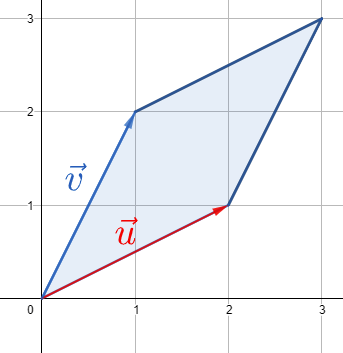
\includegraphics[width=3cm]{determinant.png}
\end{center}
On peut démontrer que l'aire orientée du parallélogramme est donnée par:  
$$
\Fonction{\det}{\R^2\times\R^2}{\R}{((x_1,y_1),(x_2,y_2))}{\begin{vmatrix}
x_1 & x_2 \\
y_1 & y_2
\end{vmatrix}=x_1y_2-y_1x_2}.
$$
Le signe du déterminant s'interprète comme le signe de l'angle orienté entre les deux vecteurs. La valeur absolue du déterminant donne l'aire du parallélogramme engendré. Ceci se révèle crucial dans
différents domaines des mathématiques, par exemple en analyse pour obtenir une formule de changement de variable pour les intégrales doubles.\\
On souhaite étendre l'application déterminant pour calculer le volume d'un parallélépipèdes défini par trois vecteurs dans l'espace : $\det(\vec{u},\vec{v},\vec{w}).$
\begin{center}
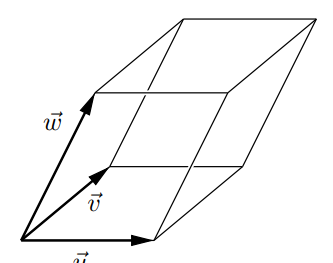
\includegraphics[width=3cm]{determinant3.png}
\end{center}
L'idée fondamentale est de prolonger l'application  déterminant dans le plan à partir de ses propriétés.\\ 
Sur le plan, on remarque que cette application est :
\begin{enumerate}
\item \defi{Normalisé} : l'aire du carré unité est 1, $\det(\vec{e_1},\vec{e_2})=1$
\item \defi{2-linéaire} : linéaire par rapport à chaque une de ces deux variables.
\begin{center}
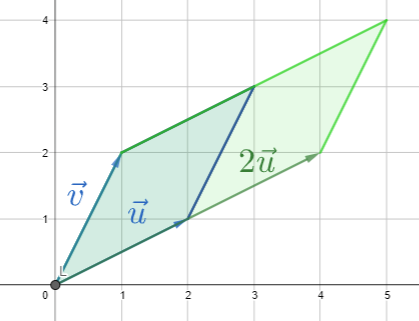
\includegraphics[width=3cm]{determinant2.png}
\end{center}
\item \defi{Alternée} : l'aire d'un parallélogramme aplati est 0, $\det(\vec{u},\vec{v})=0$ si $\vec{u}=\vec{v}.$
\end{enumerate}
Donc dans l'espace, cette application devrait être :
\begin{enumerate}
\item \defi{Normalisé} : le volume du cube unité est 1, $\det(\vec{e_1},\vec{e_2},\vec{e_3})=1$
\item \defi{3-linéaire} : linéaire par rapport à chaque une de ces trois variables.
\item \defi{Alternée} : le volume d'un parallélépipèdes aplati est 0,  $\det(\vec{u},\vec{v},\vec{w})=0$ si $\vec{u}=\vec{v}$ ou $\vec{u}=\vec{w}$ ou $\vec{v}=\vec{w}$.
\end{enumerate}
Un théorème important est qu'il existe une unique application respectant ces propriétés quelque soit la dimension.\\
Dans la suite, les vecteurs sont rangés sous forme d'une matrice, par exemple $\det((x_1,y_1),(x_2,y_2))=\det(\begin{pmatrix}
x_1 & x_2 \\
y_1 & y_2
\end{pmatrix}).$ 


%Cette \href{https://www.youtube.com/watch?v=Ip3X9LOh2dk}{vidéo de la chaine 3Blue1Brown}
% est une très bonne introduction de la notion de déterminant dans le plan et l'espace. 
 

\begin{Theoreme}[Unicité et existence du déterminant]
Soit $n\in  \N^*$.
Il existe une unique application $\det: \MnK\to\K$ vérifiant les propriétés suivantes:
\begin{enumerate}
\item $\det(\mathrm{I}_n) = 1$;
\item
  $\det(A) = 0$ si deux colonnes de $A$ sont égales;
\item
  Si on fixe $n-1$ colonnes de $A$, l'application qui à la dernière colonne associe $\det(A)$ est linéaire.
  $$\lambda \det(C_1 \dots C_i \dots C_n) + \mu  \det(C_1 \dots C'_i \dots C_n) = \det(C_1 \dots  \lambda C_i+ \mu C'_i  \dots C_n).$$
\end{enumerate}
\end{Theoreme}
\begin{Proposition}[Propriétés]
Cette application $\det$ vérifie alors automatiquement les propriétés suivantes:
\begin{enumerate}
\item \defi{antisymétrique } : 
  $$\det(C_1 \dots C_i \dots C_j  \dots C_n) = -\det(C_1 \dots C_j \dots C_i  \dots C_n)\text{ si }i\neq j$$
\item \defi{stable par combinaison linéaire} :
  $$\det(C_1 \dots C_i  \dots C_n) =\det(C_1 \dots C_i+\lambda C_j  \dots C_n)\text{ si }i\neq j$$
\item \defi{homothétie d'une colonne} :
  $$\det(C_1 \dots \lambda C_i  \dots C_n) =\lambda\det(C_1 \dots C_i  \dots C_n)$$
  En particulier,
  $$\det(\lambda A) =\lambda^n\det(A)$$
\item  \defi{stable par transposition} $$\det (A) = \det (\transposee{A})$$
\item  \defi{multiplication} $$\det (AB) = \det (A)\det(B)$$
\item  \defi{inversible}  $\det(A) \neq 0$ si et seulement si $A$ est inversible. Si $A$ est inversible, son inverse est donnée par :
$$ A^{-1}=\frac {1}{\det A} {\transposee{\text{com}A}}$$
où $\transposee{\text{com}A}$ est la transposée de la comatrice de $A$.
\end{enumerate}
Dans toutes les propriétés précédentes, on peut remplacer les opération sur les colonnes par des opération sur les lignes.
\end{Proposition}
\begin{Proposition}[Matrice triangulaire] Le déterminant d'une matrice triangulaire,$\begin{pmatrix}a_{11}&a_{12}&\cdots &\cdots &a_{1n}\\0&a_{22}&&&a_{2n}\\\vdots &\ddots &\ddots &&\vdots \\\vdots &&\ddots &\ddots &\vdots \\0&\cdots &\cdots &0&a_{nn}\\\end{pmatrix}$,  est égale au produit des coefficients de la diagonale, soit $a_{11}\times a_{22} \times\dots\times a_{nn}$.
\end{Proposition}
\begin{Definition}[Déterminant d'un endomorphisme]
Soit $E$ un $\K $-espace vectoriel de dimension finie et $u$ un endomorphisme de $E$.\\
Soit $\mathcal{B}$ une base de $E$ et $M$ la matrice de $u$ dans la base $\mathcal{B}$.\\
La quantité $\det(M)$ ne dépendant pas du choix de la base $\mathcal{B}$, mais seulement de $u$, on l'appelle \defi{déterminant} de l'endomorphisme $u$ et on note $\det(u) = \det(M)$.
\end{Definition}
\begin{Exemple}[Déterminant de Vandermonde]

Soit $a_1,\dots,a_n \in  \K ^n$.
La \defi{matrice de Vandermonde} associée à $(a_1,\dots,a_n)$ est
\[ M = \begin{pmatrix}
    1 &  1 &  1 &  \dots &  1  \\
    a_1 &  a_2 &  a_3 &  \dots &  a_n  \\
    a_1^2 &  a_2^2 &  a_3^2 &  \dots &  a_n^2  \\
    \vdots &  \vdots &  \vdots &   &  \vdots  \\
a_1^{n-1} &  a_2^{n-1} &  a_3^{n-1} &  \dots &  a_n^{n-1}  \end{pmatrix}. \]
Le \defi{déterminant de Vandermonde} $V(a_1,\dots,a_n)$ est le déterminant de la matrice de Vandermonde ci-dessus. On a :
$$V(a_1,\dots,a_n) = \prod_{1\leq i < j\leq n} (a_j - a_i). $$
En particulier,
\begin{itemize}
\item $V(a) = 1$,
\item $V(a,b) = b-a$,
\item $V(a,b,c) = (b-a)(c-a)(c-b)$.
\end{itemize}
La matrice de Vandermonde associée à $(a_1,\dots,a_n)$ est inversible si et seulement si les nombres $(a_1,\dots,a_n)$ sont deux à deux distincts.
\end{Exemple}
%TOD polynomoe caractéristique
%
%TODO compléter cette présentation succinte du détermiant...
%
%% ------------------------------------------------------------------------------
\subsection{Trace}
\begin{Definition}[Trace]
Soit $A = (a_{ij})_{1\leq i,j\leq n}\in  \MnK$ une matrice carrée.\\
La \defi{trace} de la $A$ est le scalaire
\[ \Tr(A) = \sum  _{k=1}^n a_{k k}. \]
\end{Definition}
%TODO exemple
\begin{Proposition}[Propriétés]
\begin{enumerate}
\item La trace est une application linéaire de $\MnK$ dans $\K $.
  Autrement dit, pour toutes matrices $(A,B)\in  \MnK^2$ et pour tous $(\lambda ,\mu  )\in  \K ^2$, on a
  \[ \Tr(\lambda A + \mu  B) = \lambda \Tr(A) + \mu  \Tr(B). \]
\item Pour toutes matrices $(A,B) \in  \MnK^2$, on a
  \[ \Tr(AB) = \Tr(BA). \]
\item Si $A$ et $B$ sont deux matrices semblables de $\MnK$, alors elles ont la même trace.
\end{enumerate}
\end{Proposition}
\begin{Remarque}
En général, $\Tr(ABC)\neq \Tr(ACB)$.
\end{Remarque}

\begin{Definition}[Trace d'un endomorphisme]
Soit $E$ un $\K $-espace vectoriel de dimension finie et $u$ un endomorphisme de $E$.
Soit $\mathcal{B}$ une base de $E$ et $M$ la matrice de $u$ dans la base $\mathcal{B}$.
La quantité $\Tr(M)$ ne dépendant pas du choix de la base $\mathcal{B}$, mais seulement de $u$, on l'appelle \defi{trace} de l'endomorphisme $u$ et on note $\Tr(u) = \Tr(M)$.
\end{Definition}


\begin{Proposition}[Propriétés]
\begin{enumerate}
\item La trace est une application linéaire de $\LE$ dans $\K $.
\item Si $u$ et $v$ sont deux endomorphismes de $E$, alors $\Tr(u\circ v) = \Tr(v\circ u)$.
\end{enumerate}
\end{Proposition}

\subsection{Polynôme d'endomorphismes/de matrices carrés}

\begin{Definition}[Polynôme d'endomorphismes]
Soit $u\in  \LE$ un endomorphisme.\\
On définit par récurrence $u^n$ pour $n\in  \N $ par
$u^0 = \mathrm {Id}_{E}$ et $\forall   n\in  \N $, $u^{n+1} = u\circ u^n$.\\
Pour $P = \sum  _{k=0}^d a_k X^k$, on pose $P(u) = \sum  _{k=0}^d a_k u^k$.
\end{Definition}
\begin{Definition}[Polynôme de matrices carrés]
Soit $M\in  \MnK$ une matrice carré.\\
On définit par récurrence $M^n$ pour $n\in  \N $ par
$M^0 = \mathrm {I}_{n}$ et $\forall   n\in  \N $, $M^{n+1} = M\times M^n$.\\
Pour $P = \sum  _{k=0}^d a_k X^k$, on pose $P(M) = \sum  _{k=0}^d a_k M^k$.
\end{Definition}
\begin{Proposition}[Binôme de Newton]
La formule du binôme est vérifiée quand les deux endomorphismes $u$ et $v$ commutent  :
$$(u+v)^{{n}}=\sum _{{k=0}}^{{n}}{{\binom  {n}{k}}u^{{k}}\circ v^{{n-k}}}$$
La formule du binôme est vérifiée quand les deux matrices carrés $A$ et $B$ commutent  :
$$(A+B)^{{n}}=\sum _{{k=0}}^{{n}}{{\binom  {n}{k}}A^{{k}} V^{{n-k}}}$$.
\end{Proposition}
\begin{Proposition}[Propriétés]
Soit $P$ et $Q$ sont deux polynômes et $\lambda $ un scalaire, on a
\begin{enumerate}
\item $(\lambda P)(u) = \lambda P(u)$
\item $(P+Q)(u) = P(u) + Q(u)$
\item $(PQ)(u) = P(u)\circ Q(u)$
\end{enumerate}
\end{Proposition}
\begin{Proposition}[Propriétés]
Soit $P$ et $Q$ sont deux polynômes et $\lambda $ un scalaire, on a
\begin{enumerate}
\item $(\lambda P)(M) = \lambda P(M)$
\item $(P+Q)(M) = P(M) + Q(M)$
\item $(PQ)(M) = P(M) Q(M)$
\end{enumerate}
\end{Proposition}
\begin{Proposition}[Conjugaison]
Soit $u\in  \LE$, $q\in  \GLE$ et $P\in  \K [X]$.
Alors
\[ P \bigl( q^{-1}uq \bigr) = q^{-1} \, P(u) \, q. \]
Cela implique deux endomorphisme si $u$ est semblable à $v$ alors $P(u)$ est semblable à $P(v)$.
\end{Proposition}
\begin{Proposition}[Conjugaison]
Soit $A\in  \MnK$, $Q\in  \mathcal{GL}_n(\K)$ et $P\in  \K [X]$.
Alors
\[ P \bigl( Q^{-1}u Q \bigr) = Q^{-1} \, P(u) \, Q. \]
Cela implique deux endomorphisme si $A$ est semblable à $B$ alors $P(A)$ est semblable à $P(B)$.
\end{Proposition}
\begin{Exemple}[Polynôme annulateur]
Soit $A=\begin{pmatrix}
1 &0 \\ 1&2\\
\end{pmatrix}$.\\
Montrer que le polynôme $P=(X-2)(X-1)$ annule, c'est à dire $P(A)=0$.\\
On a $A^2=\begin{pmatrix}
1 &0 \\ 3&4\\
\end{pmatrix}$. D'où $A^2-3A+2\mathrm{I}_2=0$. Soit  $(A-2\mathrm{I}_2)(A-\mathrm{I}_2)=0.$
En déduire que $\Ker(A-2\mathrm{I}_2)\oplus \Ker(A-\mathrm{I}_2)=\M{2}{1}{\R}$.\\
Analyse :
\begin{itemize}
\item  Soit $X\in \M{2}{\R}$ une matrice colonne tel que $X=Y+Z$ avec  $Y\in \Ker(A-2\mathrm{I}_2)$ ($(A-2\mathrm{I}_2)Y=0$, soit $AY=2Y$) et  $Z\in\Ker(A-\mathrm{I}_2)=\M{2}{\R}$ ($AZ=Z$).\\
On applique $A$ à l'équation $X=Y+Z$. On obtient $AX\overbrace{=}^{\text{linéarité}}AY+AZ=2Y+Z$. En combinant ces deux équations, on obtient $Y=AX-X$ et $Z=2X-AX$. Ainsi, si $Y$ et $Z$ existent, ils s'écrivent nécessairement comme ci-dessus démontrant l'unicité de la décomposition.\\
\end{itemize}
Synthèse :
\begin{itemize}
\item $AX-X\in\Ker(A-2\mathrm{I}_2)$ :  $(A-2\mathrm{I}_2)(AX-X)=(A-2\mathrm{I}_2)(A-\mathrm{I}_2)X=0X=0.$
\item $2X-AX\in\Ker(A-\mathrm{I}_2)$ :  $(A-\mathrm{I}_2)(2X-AX)=(A-\mathrm{I}_2)(A-2\mathrm{I}_2)X=0X=0.$ 
\end{itemize}
\end{Exemple}


%TODO (A-I_n)(A-2I_n)=0 

%%
%%% ---------------------------------------------------------------------------
\section{Matrices par blocs}

\begin{Definition}[Décomposition par blocs]
Soit $A\in  \MnpK $ une matrice.
Sa \defi{décomposition par blocs} suivant le découpage $(n_1,\dots,n_s) $ pour les lignes et $(p_1,\dots,p_t)$ pour les colonnes est
\begin{center}
  \begin{tikzpicture}[
      dots/.style={
        line width=1pt,
        line cap=round,
        dash pattern=on 0pt off 5pt,
        shorten >=.1cm,
    shorten <=.1cm}]
    \matrix[
      matrix of nodes,
      left delimiter=(,
      right delimiter=),
    ]{
      \node (A) {$A_{1,1}$}; &[1.1cm] \node (B) {$A_{1,t}$}; \\[1.1cm]
      \node (C) {$A_{s,1}$}; &        \node (D) {$A_{s,t}$}; \\
    };

    \draw [dots] (A.east)  -- (B.west);
    \draw [dots] (C.east)  -- (D.west);
    \draw [dots] (A.south) -- (C.north);
    \draw [dots] (B.south) -- (D.north);

    \draw [<->]  ([xshift=1cm]B.north east) -- node [right] {$n_1$} ([xshift=1cm]B.south east);
    \draw [<->]  ([xshift=1cm]D.north east) -- node [right] {$n_s$} ([xshift=1cm]D.south east);
    \draw [dots] ([xshift=1cm]B.south east) -- ([xshift=1cm]D.north east);
    \draw [<->]  ([xshift=1.75cm]B.north east) -- node [right] {$n$} ([xshift=1.75cm]D.south east);

    \draw [<->]  ([yshift=-0.5cm]C.south west) -- node [below] {$p_1$}([yshift=-0.5cm]C.south east);
    \draw [<->]  ([yshift=-0.5cm]D.south west) -- node [below] {$p_t$}([yshift=-0.5cm]D.south east);
    \draw [dots] ([yshift=-0.5cm]C.south east) -- ([yshift=-0.5cm]D.south west);
    \draw [<->]  ([yshift=-1.1cm]C.south west) -- node [below] {$p$} ([yshift=-1.1cm]D.south east);

    \node[xshift=-0.9cm] at ($(A.west)!0.5!(C.west)$) { $A =$ };
  \end{tikzpicture}
\end{center}
\end{Definition}
\begin{Exemple}
La matrice ${P} ={\begin{pmatrix}1&1&2&2\\1&1&2&2\\3&3&4&4\\3&3&4&4\end{pmatrix}}$
peut être partitionnée en quatre blocs $2\times 2$ avec $$P_{11}={\begin{pmatrix}1&1\\1&1\end{pmatrix}},P_{12}={\begin{pmatrix}2&2\\2&2\end{pmatrix}},P_{21}={\begin{pmatrix}3&3\\3&3\end{pmatrix}},{P}_{22}={\begin{pmatrix}4&4\\4&4\end{pmatrix}}.$$
On peut alors écrire la matrice par bloc comme :
$$P={\begin{pmatrix} {P} _{11}& {P} _{12}\\ {P} _{21}& {P} _{22}\end{pmatrix}}.$$
\end{Exemple}
\begin{Proposition}[Addition par blocs]
Soit $A$ et $B$ deux matrices de $\MnpK$ exprimées par blocs selon les mêmes découpages. Soit $\lambda ,\mu  \in  \K $.\\
Alors la matrice $\lambda A + \mu  B$ s'exprime par blocs selon les mêmes découpages que $A$ et $B$, et les blocs s'obtiennent en combinant les blocs situés aux mêmes places.
\end{Proposition}
\begin{Proposition}[Produit par blocs]
Soit $A\in  \MnpK$ et $B\in  \M{p}{q}{\K}$.\\
On suppose que $A$ a une décomposition par blocs suivant le découpage $(n_1,\dots,n_s)$ pour les lignes et $(p_1,\dots,n_t)$ pour les colonnes.\\
On suppose que $B$ a une décomposition par blocs suivant le découpage $(p_1,\dots,n_t)$ pour les lignes et $(q_1,\dots,q_u)$ pour les colonnes.\\
Alors le produit $C = AB\in  \mathrm{M}_{n,q}(\K )$ admet une décomposition par blocs suivant le découpage $(n_1,\dots,n_s)$ pour les lignes et $(q_1,\dots,q_u)$ pour les colonnes
\[ C = \begin{pmatrix} C_{1,1} &  \dots &  C_{1,u}  \\  \vdots &   &  \vdots  \\  C_{s,1} &  \dots &  C_{s,u} \end{pmatrix} \]
où pour tous $i\in  \{1,\dots,s\}$ et $j\in  \{1,\dots,u\}$,
\[ C_{i,j} = \sum  _{k=1}^t A_{i,k} B_{k,j} \]
\end{Proposition}
\begin{Remarque}
Le cas qui nous intéressera le plus fréquemment est celui des matrices carrées ayant le même découpage pour les lignes et pour les colonnes. Dans ce cas, les blocs diagonaux sont également des matrices carrées.
\end{Remarque}
\begin{Proposition}[Déterminant triangulaire par blocs]
Soit $A\in  \MnK$ une matrice carrée admettant une décomposition triangulaire supérieure par blocs :
$$A =\begin{pmatrix} {A} _{11}&{A} _{12}&\cdots &{A} _{1s}\\0& A_{22}&\cdots &{A} _{2s}\\\vdots &\vdots &\ddots &\vdots \\0&0&\cdots &A_{nn}\end{pmatrix}.$$
Alors $$ \det(A) = \prod_{k=1}^s \det(A_{kk}) \text{ et } \tr(A)= \sum_{k=1}^s \tr(A_{kk}) $$
\end{Proposition}

\section{Catégories d'applications linéaires}
\subsection{Forme linéaire : $E\mapsto \K $}
\begin{Definition}[Forme linéaire]

Soit $E$ un $\K $-espace vectoriel.
\begin{itemize}
\item
  Une \defi{forme linéaire} sur $E$ est une application linéaire $\Phi E\to \K $.
\item  L'ensemble des formes linéaires sur $E$ s'appelle le \defi{dual} de $E$  et se note $E^* = \mathcal{L}(E,\K )$.
\item
  Une \defi{droite} de $E$ est un sous espace vectoriel de dimension $1$.
  Autrement dit, $D$ est une droite (vectorielle) si et seulement si $\exists  \vec{x}\in  E\setminus \{\vec{0_E}\} \quad D =\K \vec{x}$.
\item
  Un \defi{hyperplan} de $E$ est un sous espace vectoriel $H$
  qui admet une droite comme supplémentaire.
  Autrement dit, si $H$ est un sous espace vectoriel de $E$,
  $H$ est un hyperplan si et seulement si  $\exists  \vec{x}\in  E\setminus \{\vec{0_E}\}$, $E = H\setminus \K \vec{x}$.
\end{itemize}
\end{Definition}
\begin{Exemple}[Équation du plan vectoriel]
Soit $P = \{(x,y,z)\in  \R ^3:2x+y-z=0\}$ un hyperplan de $\R^3$.\\
Soit $x = (1,0,0)$ et $D = \K x$. On a $E = P \oplus D$.\\
Soit $\Phi$ la forme linéaire définie par $ \Fonction{\Phi }{E}{\R }{(x,y,z)}{2x+y-z}$. On a $P = \Ker \Phi $ et $[\phi]_{\mathcal{B}}=(2,1,-1)$ avec $\mathcal{B}$ la base canonique de $\R ^3$
%2) \textit{Gradient de température} : Soit $(x,y,z)$ un élément de $\R ^3$.  Le gradient de température 
%:$$\overrightarrow {\mathbb {\nabla } }T(x,y,z)=\left({\frac {\partial T}{\partial x}}(x,y,z),{\frac {\partial T}{\partial y}}(x,y,z),{\frac {\partial T}{\partial z}}(x,y,z)\right)$$  est une forme linéaire sur l'ensemble des fonctions différentiables: $\{T:\R ^3\to \mathbb {R}: T\text{ fonction différentiable}\}$.
\end{Exemple}
\begin{Proposition} 
Soit $E$ est un $\K $-espace vectoriel de dimension finie, $\mathcal{B}=(e_1,\dots,e_n)$ une base de $E$ et $\phi\in E^*$. Alors   $$[\phi]_{\mathcal{B}}=(\phi(e_1),\phi(e_2),\dots,\phi(e_n))$$ est une matrice ligne avec $n$ composantes. Si $\phi\neq 0$, $\Rang \phi =1$ et $\Ker \phi =n-1$.
\end{Proposition}

\begin{Proposition}[Dimension]
Si $E$ est un $\K$-espace vectoriel de dimension finie, alors $\dim E^* = \dim E$.
\end{Proposition}

\begin{Theoreme}
Soit $E$ un $\K$-espace vectoriel de dimension $n\in\N^*$ et $H$ un sous espace vectoriel de $E$.\\
Les conditions suivantes sont équivalentes:
\begin{enumerate}
\item $H$ est un hyperplan, c'est à dire qu'il existe une droite $D$ telle que $E = H \oplus D$;
\item $\dim H = n - 1$;
\item il existe une forme linéaire non nulle $\phi$ telle que $H = \Ker \phi$.
\end{enumerate}
\end{Theoreme}
\begin{Remarque}
En dimension quelconque, on a encore l'équivalence entre~1 et~3.
\end{Remarque}


\begin{Proposition}
Soit $E$ un $\K $-espace vectoriel, $\Phi $ et $\Psi $ deux formes linéaires non nulles sur $E$.
Alors \[ \Ker \Phi  = \Ker \Psi  \Leftrightarrow \exists  \lambda \in  \K^*:\quad \Phi  = \lambda \Psi . \]
Autrement dit, deux formes linéaires non nulles définissent le même hyperplan si et seulement si elles sont proportionnelles.
\end{Proposition}
\begin{Remarque}
Soit $E$ un $\K $-espace vectoriel de dimension finie.  On a une correspondance bijective entre:
\begin{itemize}
\item les hyperplans sur $E$, et
\item les formes linéaires non nulles sur $E$, à multiplication par un scalaire non nul près.
\end{itemize}
\end{Remarque}

\subsection{Projecteur/Symétrie}
\subsubsection{Projecteur $p(\vec{x_1} + \vec{x_2})=\vec{x_1}$}
\begin{Definition}[Projecteur]
 Soit $E$ un $\K $-espace vectoriel et $E_1$, $E_2$ deux sous-espaces vectoriels supplémentaires dans $E$  ($E = E_1 \oplus E_2$).\\
Le \defi{projecteur} $p$ (ou la projection) sur $E_1$ parallèlement à $E_2$ est défini par:
$$\Fonction{p}{ E = E_1 \oplus E_2 }{ E}{\vec{x} = \overbrace{\vec{x_1}}^{\in E_1} + \overbrace{\vec{x_2}}^{\in E_2}}{\vec{x_1}}.$$
On dit que $p$ est un \defi{projecteur} s'il existe $E_1$ et $E_2$ deux sous-espaces vectoriels supplémentaires dans $E$ tels que
$p$ est la projection sur $E_1$ parallèlement à $E_2$.
\end{Definition}

\begin{Exemple}[Sur $\mathbb {R}^2$]
\begin{center}
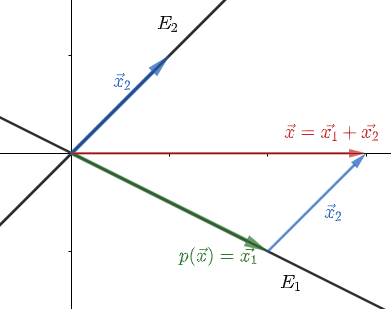
\includegraphics[width=6cm]{projecteur2d.png}
\end{center}
Cette figure ci-dessus   représente la projection, $p(\vec{x})$, du vecteur $\vec{x}=\begin{pmatrix}
3\\0
\end{pmatrix}$ sur $E_1=\mathrm{Vect}\begin{pmatrix}
2\\-1
\end{pmatrix}$ parallèlement à $E_2=\mathrm{Vect}\begin{pmatrix}
1\\1\end{pmatrix}$. Dans la base $\mathcal{B}=(\begin{pmatrix}
2\\-1
\end{pmatrix},\begin{pmatrix}
1\\1\end{pmatrix}$), on a 
$$ [p]_{\mathcal{B}} =\begin{pmatrix}1&0\\0&0\end{pmatrix}.$$
 \\
Dans $\mathbb {R}^3$, la fonction qui à $(x, y, z)$ associe $(x, y, 0)$ est la projection, $p$, sur la plan x-y parallèlement au à l'axe z. Dans la base canonique, $\mathcal{B}$, de  $\mathbb {R}^3$, on a 
$$ [p]_{\mathcal{B}}=\begin{pmatrix}1&0&0\\0&1&0\\0&0&0\end{pmatrix}.$$
\end{Exemple}
\begin{Proposition} Soit $E$ un $\K $-espace vectoriel de dimension finie, $E_1$, $E_2$ deux sous-espaces vectoriels supplémentaires dans $E$ et $\mathcal  {B}=(\overbrace{e_{1},\ldots ,e_{r}}^{\text{base de }E_1},\overbrace{e_{{r+1}},\ldots ,e_{n}}^{\text{base de }E_2})$ une base adaptée à cette décomposition.\\
Soit le projecteur $p$ sur $E_1$ parallèlement à $E_2$.\\  
Alors la matrice de $p$ dans cette base adaptée s'écrit :
$$[p]_{\mathcal{B}}=\begin{pmatrix}{\mathbf  {I}}_{{r}}&{\mathbf  {0}}\\{\mathbf  {0}}&{\mathbf  {0}}_{{n-r}}\end{pmatrix}.$$
\end{Proposition}
\begin{Proposition}[Propriétés] Soit $p$ la projection sur $E_1$ parallèlement à $E_2$. Alors:
\begin{enumerate}
\item $p \in   \LE\text{ et }p \circ p = p$
\item $\Ima p = E_1$ et $\Ker p = E_2$
\item $E_1 = \Ker(p - \mathrm{Id}_E)$ c'est-à-dire: $\vec{ x }\in   E_1 \Leftrightarrow p(\vec{x}) = \vec{x}.$ Ainsi $E_1$ est ensemble des vecteurs invariants par $p$.
\end{enumerate}
\end{Proposition}
\begin{Proposition}[Caractérisation] Supposons $p \in   \mathcal{L}(E)$ . Alors:
$$p\text{ projecteur} \Leftrightarrow p \circ p = p.$$
Dans ce cas $\Ima p$ et $\Ker p$ sont des sous-espaces vectoriels supplémentaires de $E$ et $p$ est le projecteur sur $\Ima p =
Ker(p - Id_E)$ parallèlement à $\Ker p$.
\end{Proposition}
%
%
%
%
\subsubsection{Symétrie : $s(\vec{x_1} + \vec{x_2})=\vec{x_1}-\vec{x_2}$}
\begin{Definition}[Projecteur]
 Soit $E$ un $\K $-espace vectoriel et $E_1$, $E_2$ deux sous-espaces vectoriels supplémentaires dans $E$  ($E = E_1 \oplus E_2$).\\
La \defi{symétrie} $p$ par rapport à $E_1$ parallèlement à $E_2$ est définie par:
$$\Fonction{p}{ E = E_1 \oplus E_2 }{ E}{\vec{x} = \overbrace{\vec{x_1}}^{\in E_1} + \overbrace{\vec{x_2}}^{\in E_2}}{\vec{x_1}-\vec{x_2}}.$$
On dit que $s$ est un \defi{symétrie} s'il existe $E_1$ et $E_2$ deux sous-espaces vectoriels supplémentaires dans $E$ tels que
$s$ est la symétrie  par rapport à $E_1$ parallèlement à $E_2$.
\end{Definition}
\begin{Exemple}
\begin{center}
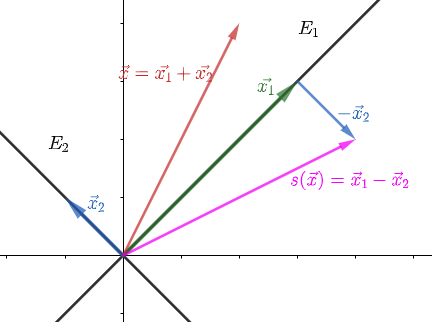
\includegraphics[width=6cm]{symetrie.png}
\end{center}
Cette figure ci-dessus représente la symétrie, $s$ par rapport à $E_1=\mathrm{Vect}\begin{pmatrix}
1\\1
\end{pmatrix}$ parallèlement à $E_2=\mathrm{Vect}\begin{pmatrix}1\\-1
\end{pmatrix}$.  Dans la base canonique $\mathcal{B}$, on a $[s]_\mathcal{B}=\begin{pmatrix}0&1\\1&0\end{pmatrix}$. En revanche dans la base  $\mathcal{B}'=\left(\begin{pmatrix}
1\\1
\end{pmatrix},\begin{pmatrix}1\\-1
\end{pmatrix}\right) $ on a $[s]_{\mathcal{B}'}=\begin{pmatrix}1&0\\0&-1\end{pmatrix}$
\end{Exemple}
\begin{Proposition}[Lien avec la projection] 
La symétrie $s$ par rapport à $E_1$ parallèlement à $E_2$ est égale à $s=2p-\mathrm{Id}_E$ avec $p$ projection sur $E_1$ parallèlement à $E_2$.
\end{Proposition}


\begin{Proposition}[Propriétés] Soit $p$ la projection sur $E_1$ parallèlement à $E_2$. Alors:
\begin{enumerate}
\item $p \in   \LE\text{ et }p \circ p = p$
\item $\Ima p = E_1$ et $\Ker p = E_2$
\item $E_1 = \Ker(p - \mathrm{Id}_E)$ c'est-à-dire: $\forall   \vec{x} \in   E,\vec{ x }\in   E_1 \Leftrightarrow p(\vec{x}) = \vec{x}.$ Ainsi $E_1$ est ensemble des vecteurs invariants par $p$.
\end{enumerate}
\end{Proposition}
\begin{Proposition}[Caractérisation] Supposons $p \in   \mathcal{L}(E)$ . Alors:
$$p\text{ projecteur} \Leftrightarrow p \circ p = p.$$
Dans ce cas $\Ima p$ et $\Ker p$ sont des sous-espaces vectoriels supplémentaires de $E$ et $p$ est le projecteur sur $\Ima p =
Ker(p - Id_E)$ parallèlement à $\Ker p$.
\end{Proposition}
\begin{Proposition}[Propriétés] Soit $s$ la symétrie par rapport à $E_1$ parallèlement à $E_2$. Alors:
\begin{enumerate}
\item $s \in   \LE\text{ et }s \circ s = \mathrm{Id}_E$
\item $\Ima s = E$ et $\Ker s = \{0_E\}$ (on retrouve le fait que $s$ est bijective)
\item $E_1 = \Ker(s - \mathrm{Id}_E)$
\item $E_2 = \Ker(s + \mathrm{Id}_E)$
\end{enumerate}
\end{Proposition}
\begin{Proposition}[Caractérisation] Supposons $s \in   \mathcal{L}(E)$ . Alors:
$$s\text{ symétrie} \Leftrightarrow s \circ s = \mathrm{Id}_E.$$
Dans ce cas $\Ker(s - \mathrm{Id}_E)$ et $\Ker(s + \mathrm{Id}_E)$ sont des sous-espaces vectoriels supplémentaires de $E$ et $s$ est la symétrie
par rapport à $\Ker(s - \mathrm{Id}_E)$ parallèlement à $\Ker(s + \mathrm{Id}_E)$.
\end{Proposition}





\section{Annexe}
\subsection{Dualité entre l'interprétation algébrique et l'interprétation algébrique}
\label{subsec:dualite}
\impo{Application linéaire en dimension finie}\\ Soit  $u\in \mathcal{L}(E,F)$ avec $E$ de dimension $p$ et $F$ de dimension $n$.\\
Soit $\mathcal{B}_E=(\vec{e_1},\dots,\vec{e_p})$ une base de $E$ et $\mathcal{B}_F=(\vec{f_1},\dots,\vec{f_n})$ une base de $F$.\\
\impo{Représentation d'un vecteur de $E$ en un vecteur colonne de $\M{M}{p,1}{\K}$}\\
Alors tout vecteur $\vec{x}$ de $E$ est déterminé de manière unique par les coefficients $\lambda_1,\dots \lambda_p$ dans le corps $\mathbb{K}$ :
$$ \vec{x}=\lambda_1.\vec{e_1}+\dots +\lambda_p.\vec{e_p}.$$
On range les coordonnées dans un vecteur colonne. 
 $$ \left[\vec{x}\right]_{\mathcal{B}_E}=\begin{pmatrix}\lambda_1\\\vdots\\\lambda_p\end{pmatrix}.$$
 L'ensemble des vecteurs colonnes est noté $\M{p}{1}{\K}$, soit l'ensemble des matrices ayant une unique colonne. On identifie les p-uplets $\mathbb{K}^p=\{(\lambda_1,\dots,\lambda_p)\}$, avec les vecteurs colonnes $\M{p}{1}{\K}=\{\begin{pmatrix}\lambda_1\\\vdots\\\lambda_p\end{pmatrix}\}$. \\
\impo{Représentation matricielle de l'application linéaire $u$}\\
Tout d'abord,  calculons l'image de chaque vecteur de la base $\mathcal{B}_E=(\vec{e_1},\dots,\vec{e_p})$ par l'application linéaire $u$ :
$$u(\vec{e_j})=a_{1j}.\vec{f_1}+\cdots +a_{nj}.\vec{f_n}\text{ avec } 1\leq j \leq p.$$
On range les coefficient, $a_{i,j}$ dans un tableau de taille $(n,p)$, noté $\left[u\right]_{\mathcal{B}_E}^{\mathcal{B}_F}$, que l'on appelle \impo{matrice} :
\begin{center}
  \begin{tikzpicture}[
      every left delimiter/.style={xshift=0.75em},
      every right delimiter/.style={xshift=-0.75em},
      dots/.style={
        line width=1pt,
        line cap=round,
        dash pattern=on 0pt off 5pt,
        shorten >=.1cm,
    shorten <=.1cm}]
    \matrix (M) [
      matrix of nodes,
      left delimiter=(,
      right delimiter=),
    ]{
      \node (A) {$a_{11}$}; &[1.1cm] \node (B) {$a_{1p}$}; \\[1.1cm]
      \node (C) {$a_{n1}$}; &        \node (D) {$a_{np}$}; \\
    };

    \draw (M.west) node[left] {$\left[u\right]_{\mathcal{B}_E}^{\mathcal{B}_F}=$};
    \draw [dots] (A.east)  -- (B.west);
    \draw [dots] (C.east)  -- (D.west);
    \draw [dots] (A.south) -- (C.north);
    \draw [dots] (B.south) -- (D.north);
    \draw (A) [yshift=0.7cm] node (E) {$u(\vec{e_1})$};
    \draw (B) [yshift=0.7cm] node (F) {$u(\vec{e_p})$};
    \draw (B) [xshift=1cm]   node (G) {$\vec{f_1}$};
    \draw (D) [xshift=1cm]   node (H) {$\vec{f_n}$};
    \draw [dots] (E.east)  -- (F.west);
    \draw [dots] (G.south) -- (H.north);
  \end{tikzpicture}.
\end{center}
\impo{Caractérisation de l'application linéaire $u$}\\
Comme $u$ est linéaire, on a :
\begin{align}
u(\vec{x})&=u(\lambda_1.\vec{e_1}+\dots +\lambda_p.\vec{e_p})\\
u(\vec{x})&=\lambda_1.u(\vec{e_1})+\dots +\lambda_p.u(\vec{e_p})
\end{align}
Cela implique que l'application linéaire $u$ est entièrement déterminée par les vecteurs :
$(u(\vec{e_1}),\dots,u(\vec{e_p}))$\\
\impo{Représentation du vecteur $u(\vec{x})$ de $F$ en un vecteur colonne $\M{M}{n,1}{\K}$}\\
Substituons $u(\vec{e_j})$ par $a_{1j}.\vec{f_1}+\cdots +a_{nj}.\vec{f_n}$ dans l'équation précédente, ce qui donne après réorganisation des termes :
\begin{align}
u(\vec{x})=& (a_{11}.\lambda_1+\dots+a_{1p}.\lambda_p).\vec{f_1}+\cdots \\
        &+(a_{n1}.\lambda_1+\dots+a_{np}.\lambda_p).\vec{f_n}.
\end{align}        
Donc, l'application linéaire $u$ est entièrement déterminée par les coefficient $a_{ij}$. On range les coordonnées du vecteur $u(\vec{x})$  dans un vecteur colonne $\M{n}{1}{\K}$:      
$$\left[u(\vec{x})\right]_{\mathcal{B}_F}=\begin{pmatrix}a_{11}.\lambda_1+\dots+a_{1p}.\lambda_p\\ \vdots\\a_{n1}.\lambda_1+\dots+a_{np}.\lambda_p\end{pmatrix}.$$
Chaque coordonné du vecteur colonne $\left[u(\vec{x})\right]_{\mathcal{B}_F}$ est la multiplication terme par terme entre les coefficients de la $i$-ème ligne de $\left[u\right]_{\mathcal{B}_E}^{\mathcal{B}_F}$ et les coefficients de la colonne $\left[\vec{x}\right]_{\mathcal{B}_E}$ : 
$$\begin{aligned}
\left[u(\vec{x})\right]_{\mathcal{B}_F} =  \left[u\right]_{\mathcal{B}_E}^{\mathcal{B}_F} \times&\left[\vec{x}\right]_{\mathcal{B}_E} \\
& \begin{pmatrix}\lambda_1\\\vdots\\\lambda_p\end{pmatrix} \\
\left[u(\vec{x})\right]_{\mathcal{B}_F}=\begin{pmatrix}
    a_{11} &  \dots & a_{1p}  \\
    \vdots &   &  \vdots  \\
    a_{n1} &  \dots & a_{np}
  \end{pmatrix}& \\
 \left[u(\vec{x})\right]_{\mathcal{B}_F}=\begin{pmatrix}a_{11}.\lambda_1+\dots+a_{1p}.\lambda_p\\\vdots\\a_{n1}.\lambda_1+\dots+a_{np}.\lambda_p\end{pmatrix}&.
\end{aligned}$$
En conclusion, pour calculer l'image d'un vecteur $\vec{x}$ par l'application linéaire $u$, il suffit de faire des multiplications et des additions entre coefficients. \\
\impo{Représentation matricielle de la composition d'applications linéaires $v\circ u$}\\
Soit $v$ une application linéaire de $F$ dans $G$. On cherche une représentation matricielle de $v\circ u$. Soit $A=\left[u\right]_{\mathcal{B}_E}^{\mathcal{B}_F}$, $B=\left[u\right]_{\mathcal{B}_F}^{\mathcal{B}_G}$ et $C=\left[v\circ u\right]_{\mathcal{B}_E}^{\mathcal{B}_G}$, que l'on note $C=B\times A$. On cherche donc à définir la multiplication entre deux matrices. Le coefficient  $c_{ij}$ de la matrice $C$ est la $j$-coordonnée du vecteur $C\times [e_i]_{\mathcal{B}_E}$, soit :  
$$\begin{aligned}
&\begin{pmatrix}0\\\vdots\\0\\1\\0\\\vdots\\0\end{pmatrix}  \\
\begin{pmatrix}
    c_{11} &  \dots & c_{1m}  \\
    \vdots &   &  \vdots  \\
    c_{n1} &  \dots & c_{nm}
  \end{pmatrix}& &=\begin{pmatrix}c_{1j}\\\vdots\\c_{nj}\end{pmatrix}
\end{aligned}$$
Comme $ (v\circ u)(e_i)=v(u(e_i))$, on a $C\times[e_i]_{\mathcal{B}_E} = B\times(A\times [e_i]_{\mathcal{B}_E})$. Donc on applique d'abord la matrice $A$ :
$$\begin{aligned}
&\begin{pmatrix}0\\\vdots\\1\\\vdots\\0\end{pmatrix}&\\   
\begin{pmatrix}
    a_{11} &  \dots & a_{1p}  \\
    \vdots &   &  \vdots  \\
    a_{n1} &  \dots & a_{np}
  \end{pmatrix}& &=\begin{pmatrix}a_{1j}\\\vdots\\a_{nj}\end{pmatrix}
\end{aligned}$$
puis la matrice $B$,
$$\begin{aligned}
&\begin{pmatrix}a_{1j}\\\vdots\\a_{nj}\end{pmatrix}&\\   
\begin{pmatrix}
    b_{11} &  \dots & b_{1n}  \\
    \vdots &   &  \vdots  \\
    b_{m1} &  \dots & b_{mn}
  \end{pmatrix}& &=\begin{pmatrix}b_{1,1}a_{1j}+\cdots +b_{1n}a_{nj}\\\vdots\\b_{m1}a_{1j}+\cdots +b_{mn}a_{pn}\end{pmatrix}
\end{aligned}$$
par identification, on obtient $c_{ij}=b_{i1}a_{1j}+\cdots +b_{in}a_{nj}=\sum _{k=1}^{n}b_{ik}a_{kj}$, soit la multiplication terme à terme des coefficients de la  i-ème ligne de $B$ et de j-ème colonne de $A$,et la somme de ces produits. Un schéma de ce produit est :  
\begin{center}

\includegraphics[width=3cm]{product_matriciel.png}
\end{center}
%\impo{Représentation d'une matrice par une application linéaire}
%Inversement, si l'on se donne une matrice $A$,
%on peut définir une application linéaire, dite \defi{canoniquement associée à $A$}, par
%\[ \Fonction{f_A}{\M{M}{p,1}{\K}}{\M{M}{n,1}{\K}}{X}{A\times X}.\]
%
%
\begin{Exemple}{Rotation}
L'application linéaire rotation d'angle $\theta$ définie par :$$\Fonction{R_\theta}{\mathbb {R}^2 }{\mathbb {R}^2}{(x,y)}{ (x\cos \theta - y \sin \theta,x\sin \theta + y \cos \theta)}$$
\begin{center}
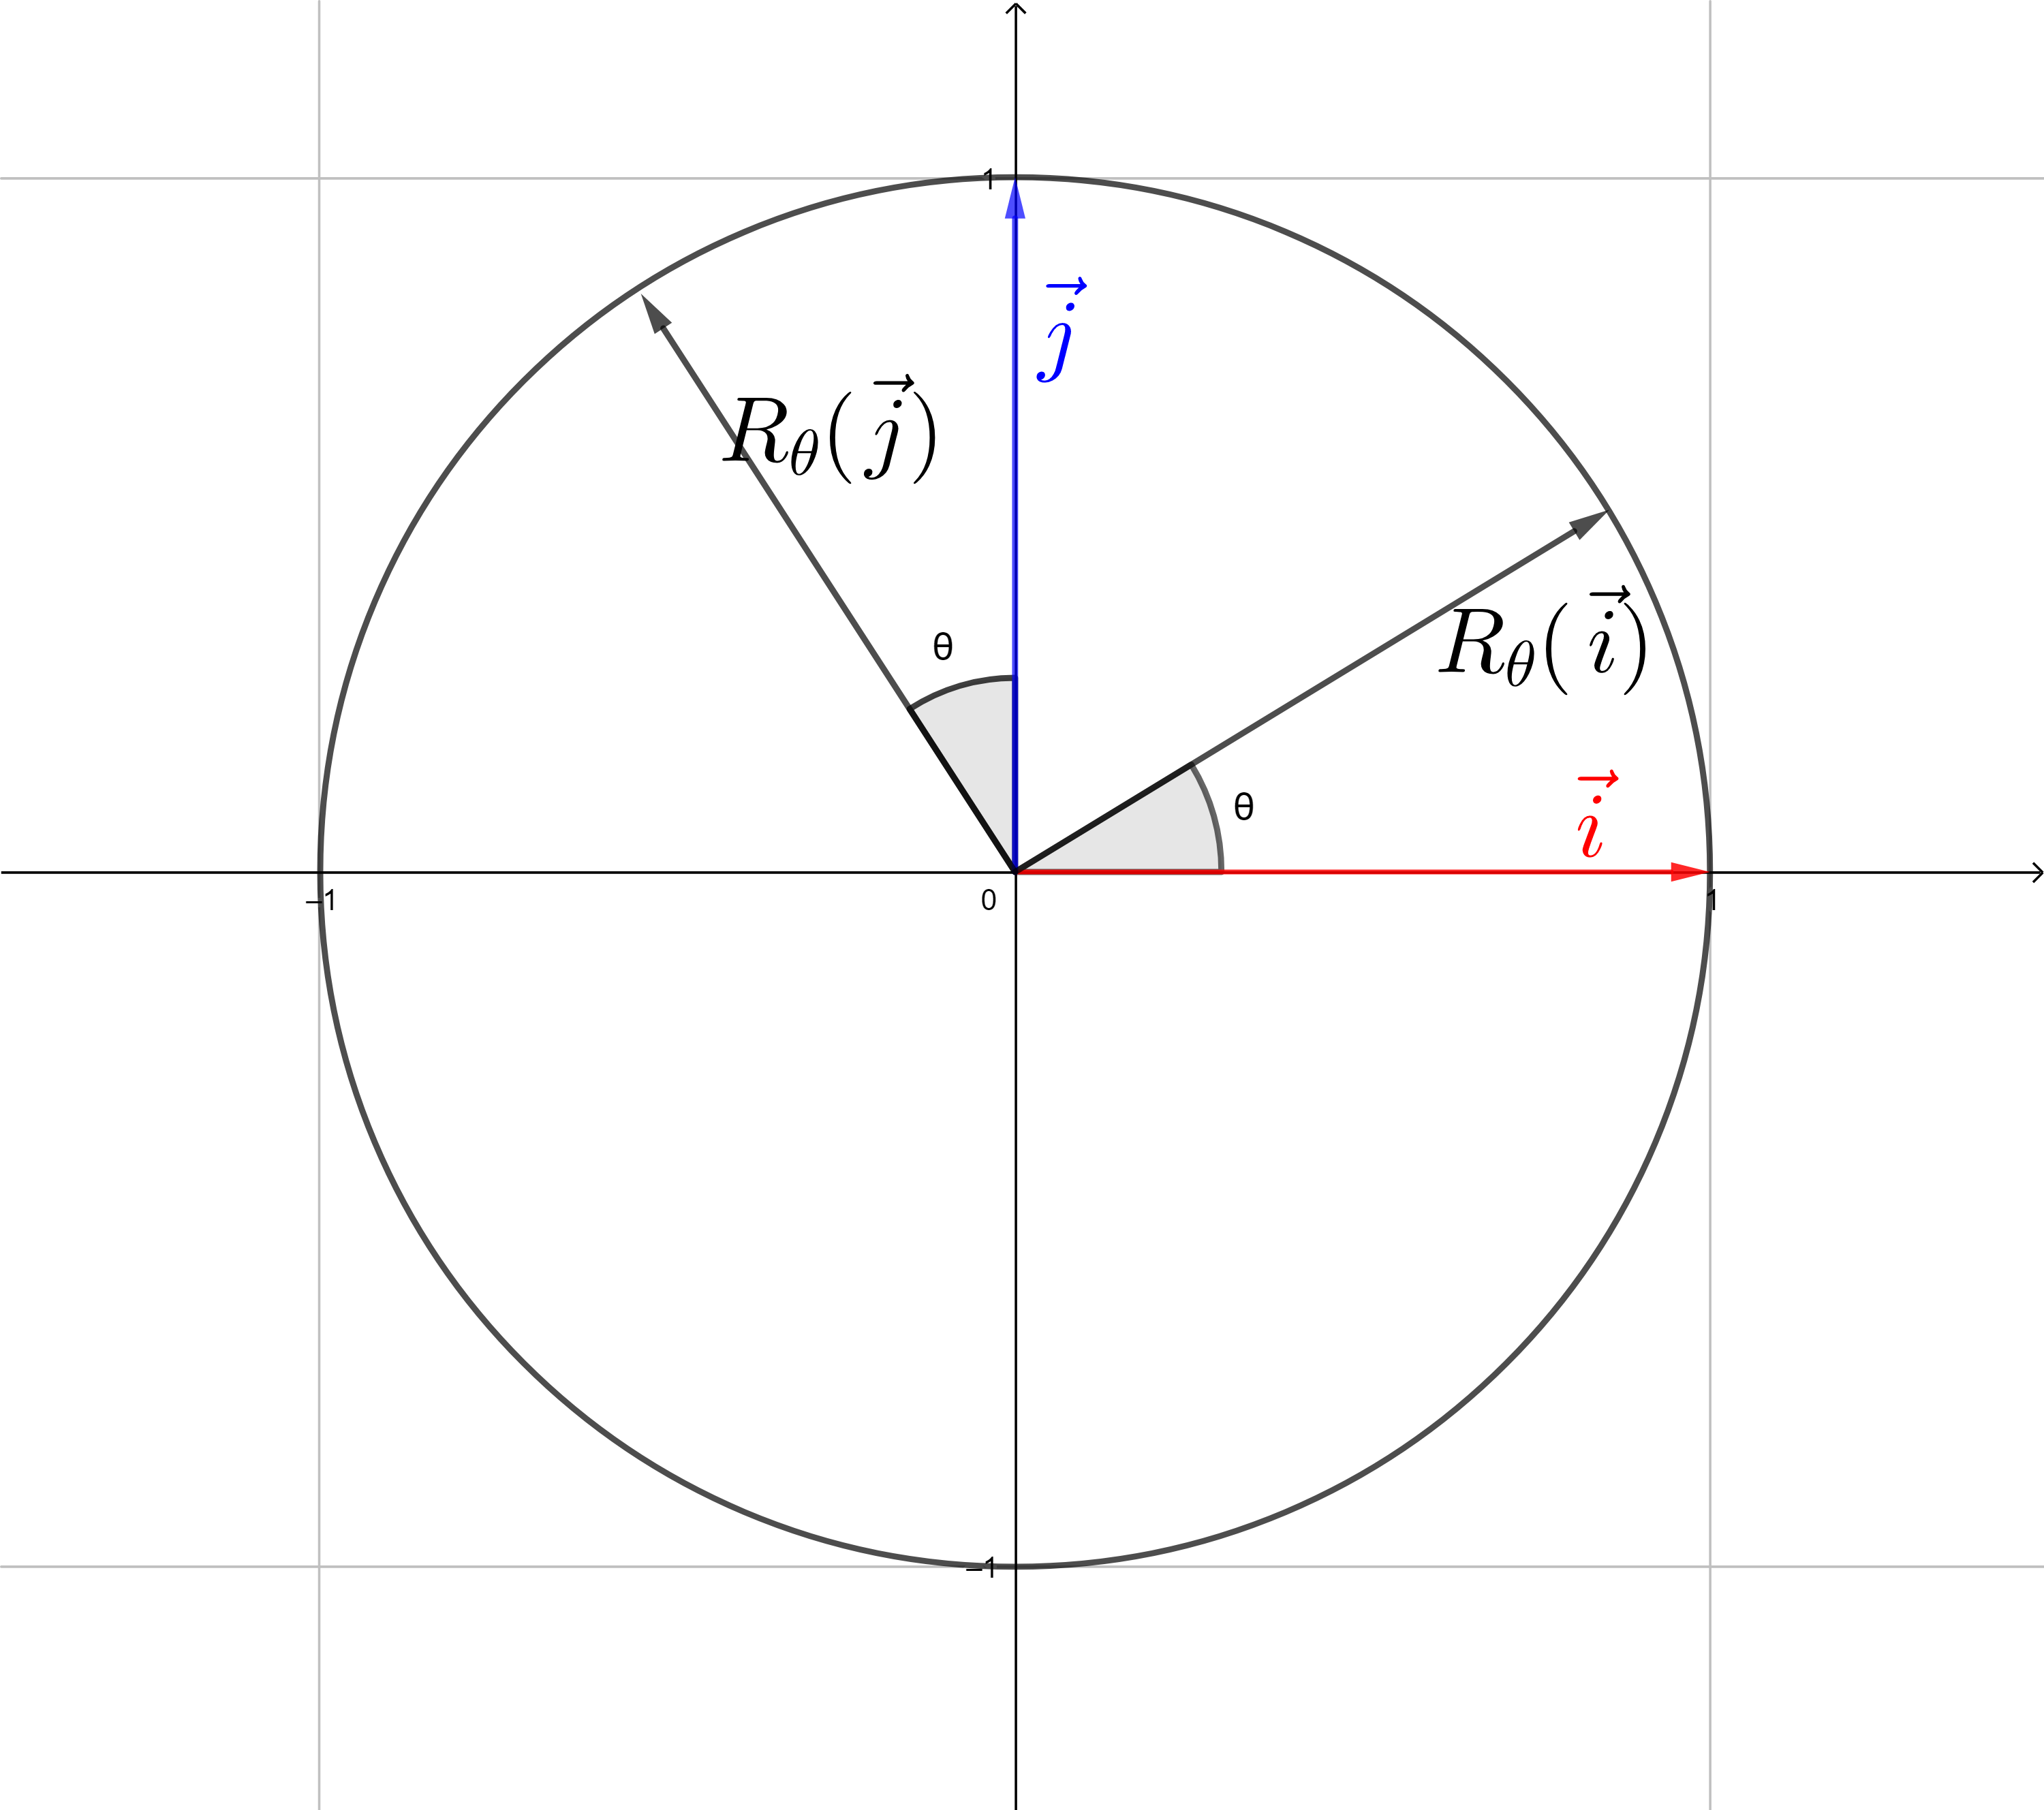
\includegraphics[width=5cm]{rotation.png}
\end{center}
En prenant la base canonique $\mathcal{B}=(\vec{i}=(1,0),\vec{j}=(0,1))$, pour base de l'espace vectoriel de départ et d'arrivé, comme $R_\theta(\vec{i})=\cos \theta \vec{i} + \sin \theta \vec{j}$ et $R_\theta(\vec{j})=-\sin \theta\vec{i}+ \cos \theta\vec{j}$, on a :

$$ [R_\theta]_\mathcal{B}=\begin{pmatrix}\cos \theta &-\sin \theta \\\sin \theta &\cos \theta\end{pmatrix}.$$
Si l'on compose deux matrice de rotation d'angle $\theta$ et $\theta'$, on a :
$$\begin{aligned}
[R_\theta]_\mathcal{B}\times[R_{\theta'}]_\mathcal{B}=\begin{pmatrix}\cos \theta &-\sin \theta \\\sin \theta &\cos \theta\end{pmatrix}\times \begin{pmatrix}\cos \theta' &-\sin \theta' \\\sin \theta' &\cos \theta'\end{pmatrix}\\
=\begin{pmatrix}\cos \theta\cos\theta'-\sin \theta\sin\theta'  &-\cos \theta\sin\theta'-\sin \theta\cos\theta' \\
\cos \theta\sin\theta'+\sin \theta\cos\theta'&\cos \theta\cos\theta'-\sin \theta\sin\theta' 
\end{pmatrix}\\
=\begin{pmatrix}\cos( \theta+\theta') &-\sin( \theta+\theta') \\\sin( \theta+\theta') &\cos( \theta+\theta')\end{pmatrix}
\end{aligned}$$ 
Donc la composition de deux rotations est une rotation d'angle la somme des angles des deux rotations.
\end{Exemple}
\subsection{Exercice de synthèse: endomorphisme sur $\R _2[X]$}
Soit $\mathbb R_2[X]$ l'espace vectoriel des polynômes à coefficients réels de degré inférieur ou égal à 2.
On définit l'application $\phi$ par : 
$$
\Fonction{\phi}{\R _2[X]}{\R _2[X]}{P}{P-P'}
$$ où $P'$ est le polynôme dérivé de $P$.
\begin{enumerate}
\item Démontrer que $\phi$ est un endomorphisme. 
\item  Démontrer que $\phi$ est un automorphisme de $\mathbb R_2[X]$.
\item Déterminer l'inverse de $\phi$.
\end{enumerate}
Correction :
\begin{enumerate}
\item 2 solutions :
\begin{enumerate}
\item 
\begin{itemize}
\item \textit{Définie} : L'application $\phi$ est bien définie car $deg(P-P')\leq deg(P)$.
\item \textit{Linéaire} : soit $P,Q\in \mathbb R_2[X]$ et soit $\lambda,\mu \in \R $.\\
$$\phi(\lambda P + \mu Q)= (\lambda P + \mu Q)-(\lambda P + \mu Q)'=\lambda (P - P')+\mu(Q - Q')= \lambda\phi( P) + \mu \phi(Q) $$
\end{itemize} 
\item Les applications, identité $\mathrm{Id}_{\R _2[X]}:P\mapsto P$ et dérivée $\psi:P\mapsto P'$, sont linéaires. Comme $\mathcal{L}(R_2[X])$ est un espace vectoriel, $\phi$ est une application linéaire car combinaison linéaire de $\mathrm{Id}_{\R _2[X]}$ et $\psi$. 
\end{enumerate}
\item 2 solutions :
\begin{enumerate}
\item Comme $\phi$ est un endomorphisme d'un espace vectoriel de dimension finie, il suffit de démontrer que  $\phi$ est injective, soit  $\Ker\phi=\{0_{\R _2[X]} \}$ .\\
Montrons que  $\{0_{\R _2[X]} \} \subset \Ker\phi $.\\
\hspace{1cm}$\Ker\phi$ est un espace vectoriel donc il contient l'élément neutre.\\
Montrons que $\Ker\phi   \subset \{0_{\R _2[X]} \}$.\\
\hspace{1cm}Soit $P\in \Ker\phi$, c'est à dire que $\phi(P)=0_{\R _2[X]}$. Soit $P=P'$. D'où $P=0_{\R _2[X]}$.
\item  Déterminons la matrice de l'endomorphisme de $\phi$ dans la base canonique, $\mathcal{B}=(1,X,X^2)$ de $\R _2[X]$.
$$[\phi]_{\mathcal{B}}=\begin{pmatrix}1 &-1&0\\0 &1&-2\\0&0&1 \end{pmatrix}\text{ car } \phi(X^i)=X^i-i  X^{i-1}.$$
Comme $\det ([\phi]_{\mathcal{B}})=1$, produit des coefficients de la diagonale pour une matrice triangulaire supérieur,  $[\phi]_{\mathcal{B}}$ est inversible, donc $\phi$ est bijectif.  
\end{enumerate}
\item 2 solutions :
\begin{enumerate}
\item L'application dérivée $\psi:P\mapsto P'$, est nilpotente car $\psi^3=0$. Comme $\psi$ et $\mathrm{Id}_{\R _2[X]}$ commutent,
on a$$ \mathrm{Id}_{\R _2[X]}=\mathrm{Id}^3_{\R _2[X]}-\psi^3=(\mathrm{Id}_{\R _2[X]}-\psi)\circ(\mathrm{Id}_{\R _2[X]}+\psi+\psi^2)=\phi\circ (\mathrm{Id}_{\R _2[X]}+\psi+\psi^2).$$ Donc l'inverse de $\phi$ est $\phi^{-1}=(\mathrm{Id}_{\R _2[X]}+\psi+\psi^2)$.
\item  Déterminons l'inverse de matrice de l'endomorphisme de $\phi$ par la méthode du pivot de Gauss:
$$\begin{array}{rl}
&\left({\begin{array}{rrr|rrr}1 &-1&0&1&0&0\\0 &1&-2&0&1&0\\0&0&1&0&0&1 \end{array}}\right)\\
\begin{small}\begin{array}{r} \\(L2)\leftarrow (L2)+2(L3) \end{array}\end{small}&\left({\begin{array}{rrr|rrr}1 &-1&0&1&0&0\\0 &1&0&0&1&2\\0&0&1&0&0&1 \end{array}}\right)\\
\begin{small}\begin{array}{r} \\(L1)\leftarrow (L1)+(L2) \end{array}\end{small}&\left({\begin{array}{rrr|rrr}1 &0&0&1&1&2\\0 &1&0&0&1&2\\0&0&1&0&0&1 \end{array}}\right)
\end{array}.$$
D'où $\phi^{-1}(1)=1,\phi^{-1}(X)=1+X$ et $\phi^{-1}(X^2)=2+2X+X^2$.  Soit $\phi^{-1}=(\mathrm{Id}_{\R _2[X]}+\psi+\psi^2)$.
\end{enumerate}
\end{enumerate}
%
%%Ne pas oublier le changement de base dans la base des vecteurs propres
%
%
%


\end{document}
